%!TEX root = spadini_davide.tex

\chapter{Evaluation}
\label{cha:evaluation}
We now want to evaluate our implementation of the \ac{WPSS} algorithm, and compare what we obtain with the original papers~\cite{wormhole} in order to confirm or contest their results. We tested our implementation both in deployment and in emulation, however due to the low number of nodes in the real environment we report only the results obtained in emulation. We want to show that our implementation provides the desirable PSS properties, such as fresh samples, randomness, and low cost in a real environment, but also we want to test robustness under different level of churn.

The structure is shown in Figure~\ref{fig:overlay}, the base overlay is a random undirected graph that is also NAT-friendly, where private nodes are connected to public nodes, and public nodes are connected to one another. The bootstrap service component provides addresses of random public nodes that are used to build the base overlay and to create wormholes. It is implemented as a central server, the tracker. The base overlay service strives to keep the overlay connected repairing broken links, thus maintaining a fixed number of outgoing links at each node. Every node maintains 20 links to random public nodes, but since these links are bidirectional, the effective average degree is 40. 

We set $TTL = 100$. As discussed in~\cite{wormhole} and also as we will see later, \ac{WPSS} messages will always terminate much sooner in most practical settings, so the TTL is not a critical parameter.

\section{Experimental Setup}
\label{sec:exp_setup}
For what concerns emulations, we implemented \ac{WPSS} using the \textbf{Hivejs-Framework-Sim} provided by the Hive Streaming company. It is very configurable, and it allows us to define the network size, the bandwidth of the nodes but also to test the implementation under different level of churn or latency. All experiments are averaged over 4 runs. We applied the same settings as in the original paper, which are: 

\begin{itemize}
	\item the view size (the number of freshest random samples a node remembers) is set to 50
	\item we set $\Delta = 1$ second
	\item we use a scenario of $N = 1000$ nodes that join following a Poisson distribution with a mean inter-arrival time of 100 milliseconds
\end{itemize}

In all the emulations 20\% of the nodes is public and 80\% is private, which, according to~\cite{wormhole}, reflects the distribution observed in the commercial deployments of their P2P application.

\section{Freshness}
\label{sec:eval_freshness}
In this experiment we want to measure the freshness of the samples using the average hop count but also the \textit{$90^{th}$} and \textit{$99^{th}$} percentiles. This is the same test reported in~\cite{wormhole}. Figure~\ref{fig:my_average_hop_count} shows our result, while in Figure~\ref{fig:paper_average_hop_count} shows their test. As we can see the result is almost identical, this means that our implementation does not alter this property. In the figure we can notice that the average hop count and the $90^{th}$ percentile grow slowly with increasing of $\Delta_{wh}$, which is the wormhole renewal timer, while the $99^{th}$ percentile grows more quickly. This was expected, since the higher the timer, the more nodes the advertisement will need to traverse in order to find a node which does not already have its sample. An important fact to notice is that the \textit{TTL} is never reached, actually in the worst case it is not greater then 20. We can notice that the performance is optimal for $\Delta_{wh}$  between about 5 and 10 seconds, as in their result. Given this finding, we set $\Delta_{wh} = 10$ for the remaining experiments, as this value has good freshness (even considering the $99^{th}$ percentile), while the number of new links required is relatively low (a new connection every 10 rounds of the algorithm). 

\begin{figure}
\centering
\begin{subfigure}{.5\textwidth}
  \centering
  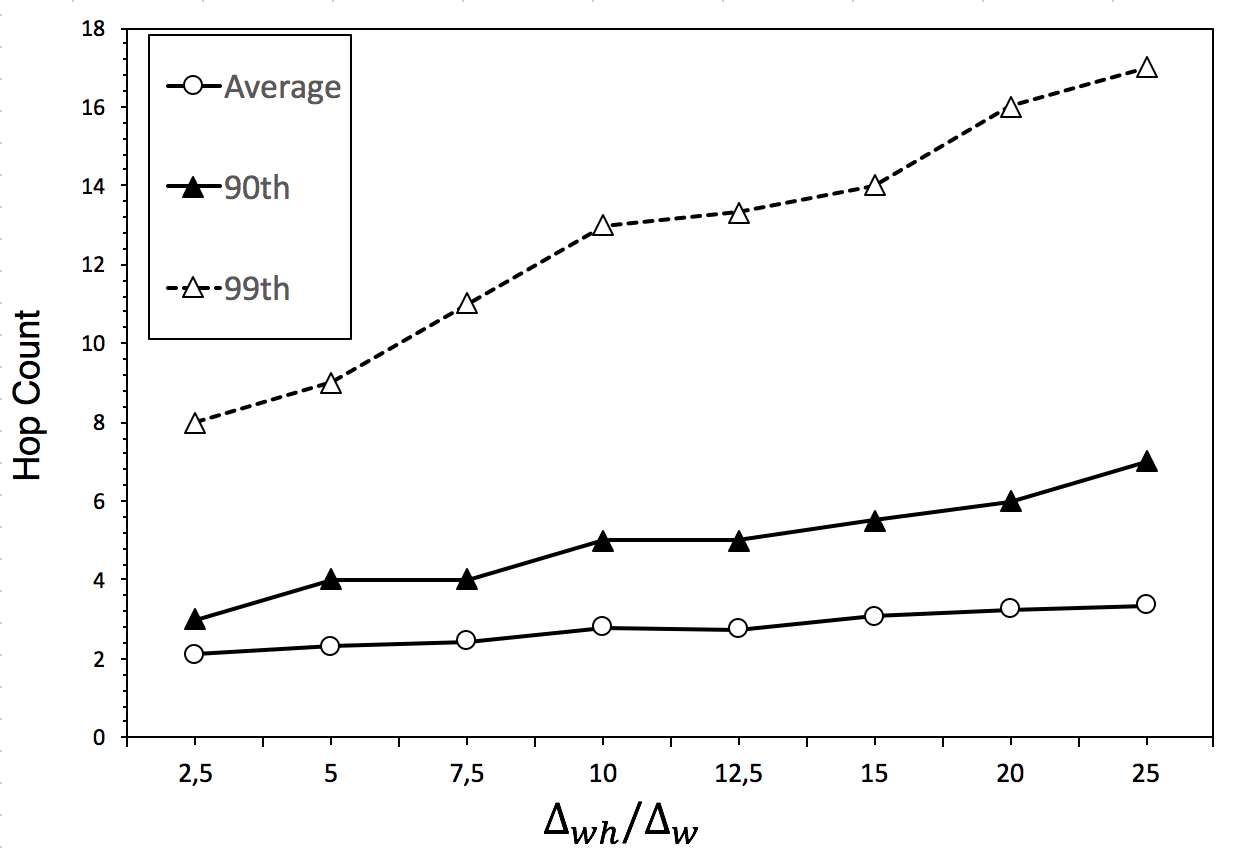
\includegraphics[keepaspectratio=true, width=1\linewidth]{images/average_hop_count}
  \caption{}
  \label{fig:my_average_hop_count}
\end{subfigure}%
\begin{subfigure}{.5\textwidth}
  \centering
  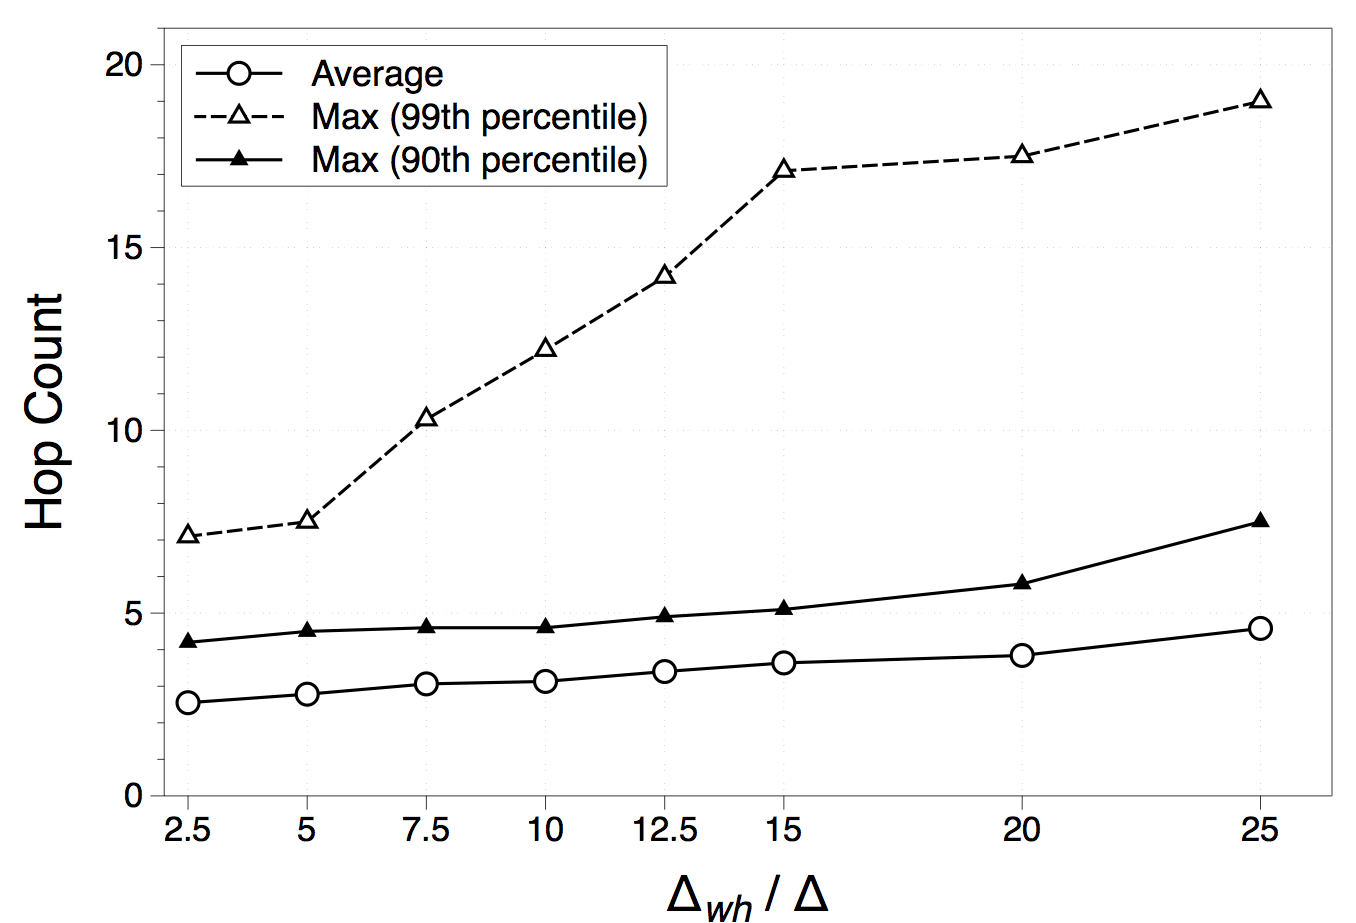
\includegraphics[keepaspectratio=true, width=1\linewidth]{images/paper_average_hop_count}
  \caption{}
  \label{fig:paper_average_hop_count}
\end{subfigure}
\caption{Measure of the average hop count, as well as the $90^{th}$ and $99^{th}$ percentile.~\ref{fig:my_average_hop_count} represents our result,~\ref{fig:paper_average_hop_count} is the test reported in the paper.}
\label{fig:freshness}
\end{figure}


\section{Randomness}
\label{sec:eval_randomness}
As in~\cite{wormhole}, we now want to evaluate the global randomness properties of our system by measuring properties of the \ac{WPSS} overlay topology, so the upper overlay. This overlay is built by the peers connecting to all the samples stored in their views. In this set of experiments, we measure the in-degree distribution of the \ac{WPSS} overlay network, its convergence time for different view sizes, and finally its clustering coefficient for different view sizes. In Figure~\ref{fig:converged_indegree} we can see the converged in-degree distribution. This test measures the in-degree of a node in the wormhole overlay, which is the number of nodes that are connected to it through this overlay. This result shows that all the nodes have an in-degree included between 43 and 64, which is almost the same result illustrated in the paper. We can notice that our result is even narrower than the original, which suggests good load balancing. 

\begin{figure}
\centering
\begin{subfigure}{.5\textwidth}
  \centering
  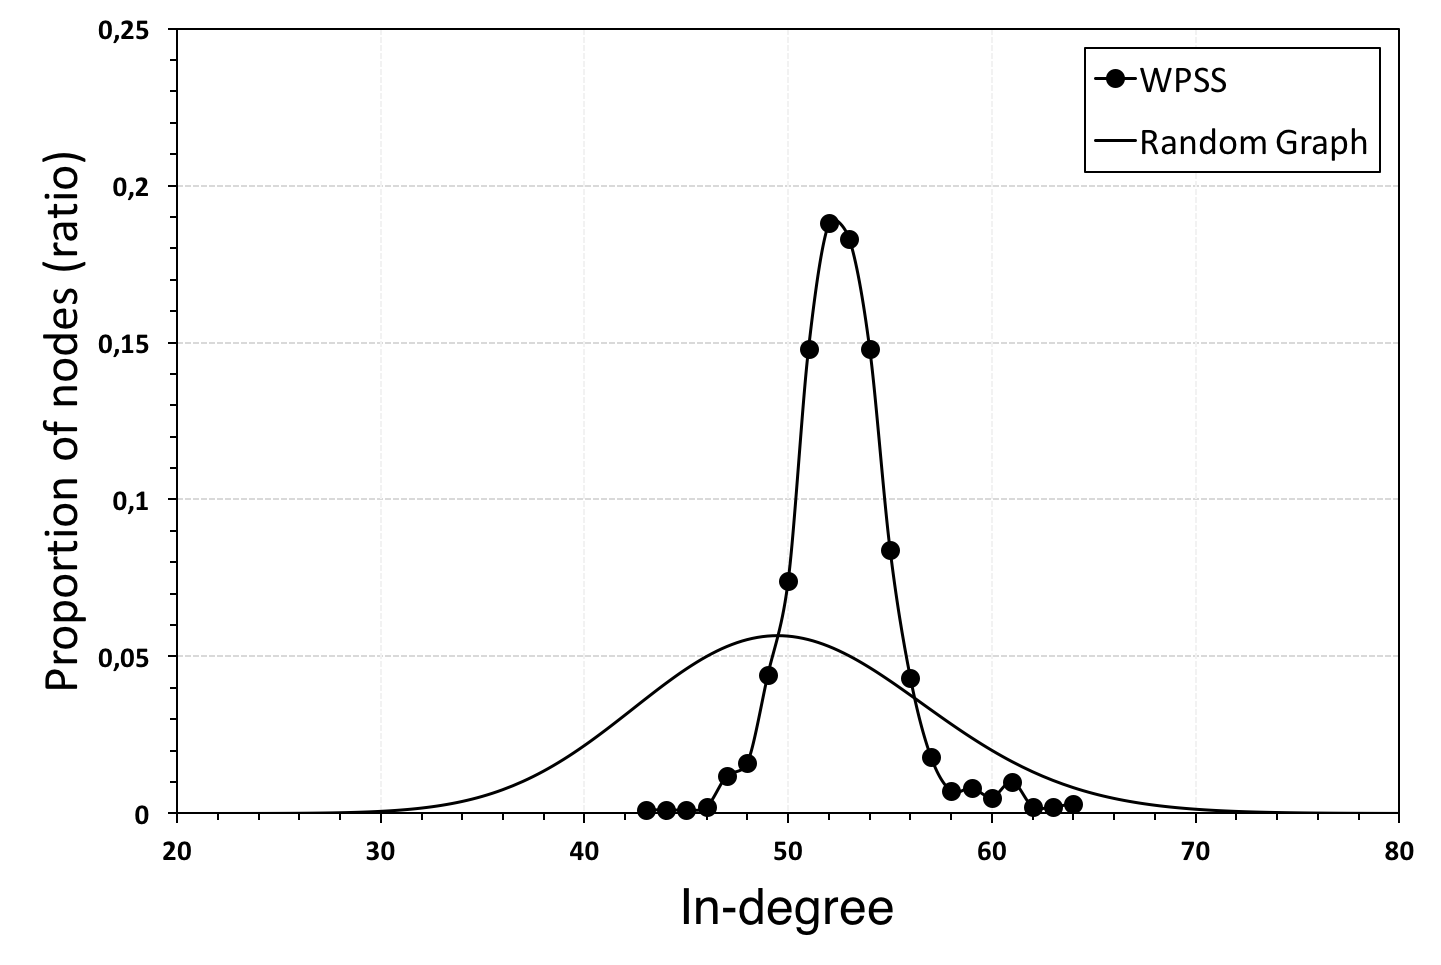
\includegraphics[keepaspectratio=true, width=1\linewidth]{images/converged_indegree}
  \caption{}
  \label{fig:converged_indegree}
\end{subfigure}%
\begin{subfigure}{.5\textwidth}
  \centering
  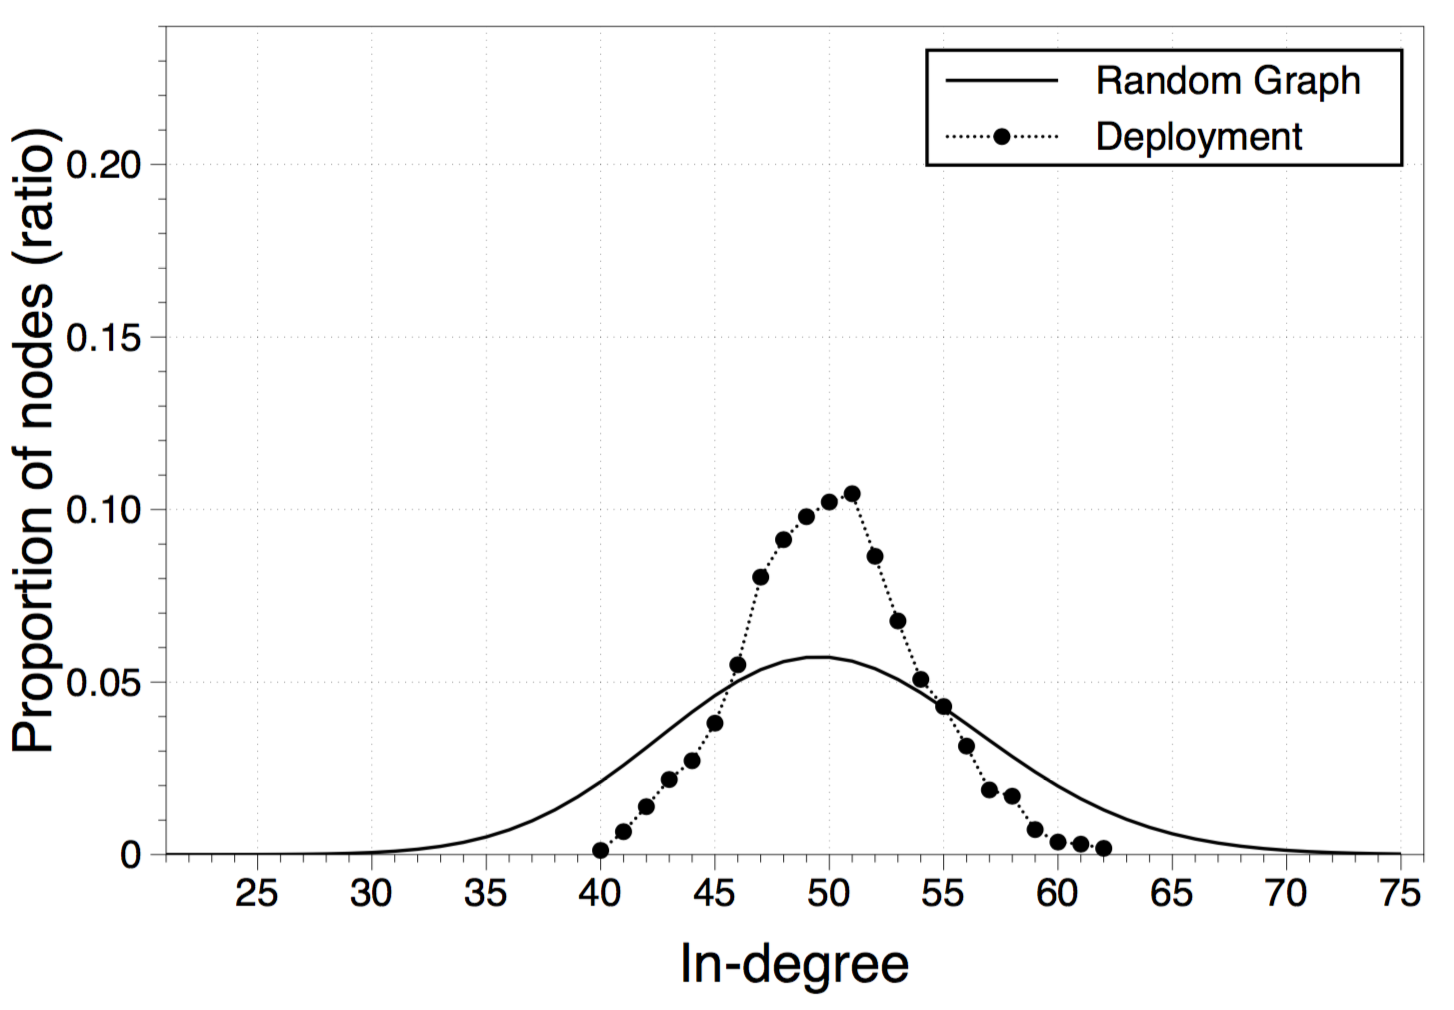
\includegraphics[keepaspectratio=true, width=1\linewidth]{images/paper_converged_indegree}
  \caption{}
  \label{fig:paper_converged_indegree}
\end{subfigure}
\caption{Converged in-degree distribution.~\ref{fig:converged_indegree} represents our result,~\ref{fig:paper_converged_indegree} is the test reported in the paper.}
\label{fig:randomness_conv_indegree}
\end{figure}

\newpage
One interesting fact, is shown in Figure~\ref{fig:indegree_evolution}: as we can see the in-degree converges to 50 after 4 minutes, and the standard deviation after 8 minutes, which are exactly the same results of the original paper, shown in Figure~\ref{fig:paper_indegree_evolution}. This is a good result, it reflects exactly what we obtained in the previous test and it means that almost all the nodes are ``known'' in the network by the same number of peers.

\begin{figure}
\centering
\begin{subfigure}{.5\textwidth}
  \centering
  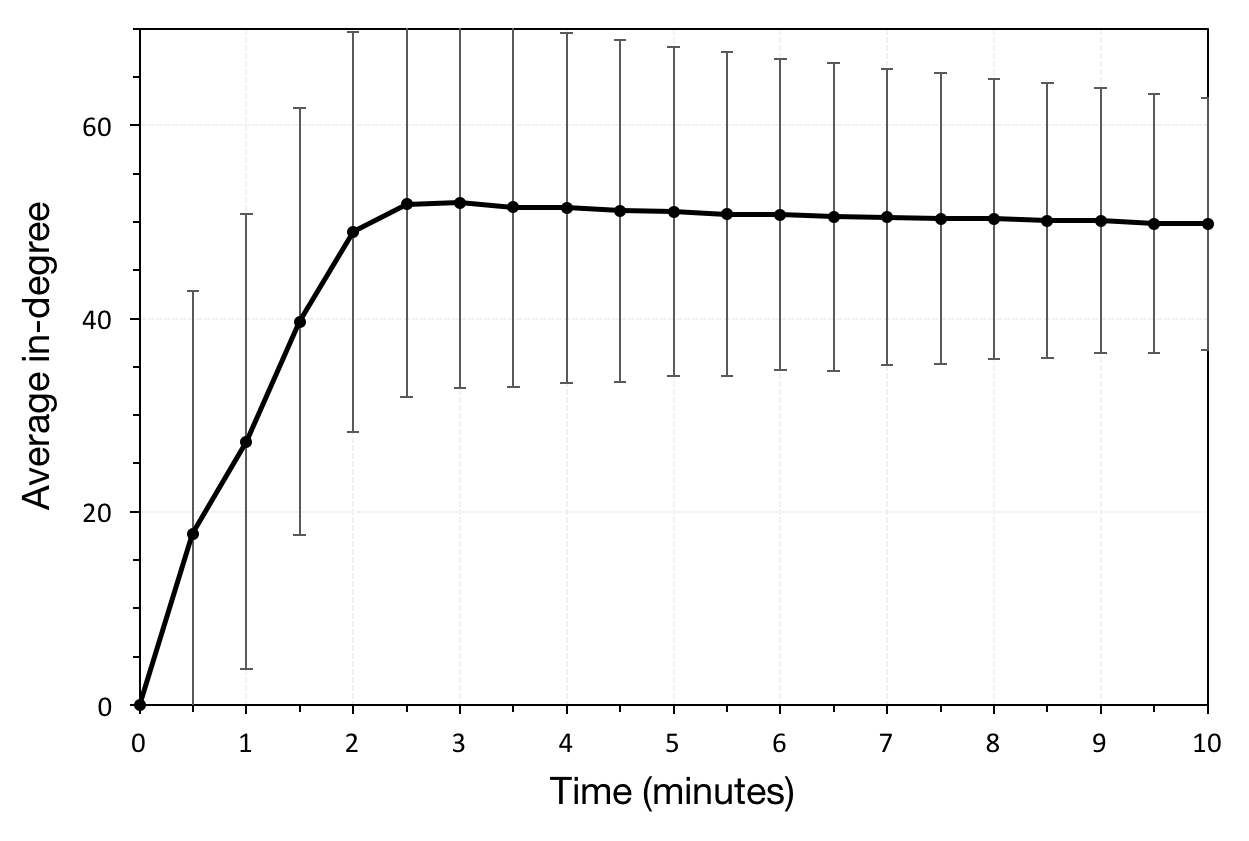
\includegraphics[keepaspectratio=true, width=1\linewidth]{images/indegree_evolution}
  \caption{}
  \label{fig:indegree_evolution}
\end{subfigure}%
\begin{subfigure}{.5\textwidth}
  \centering
  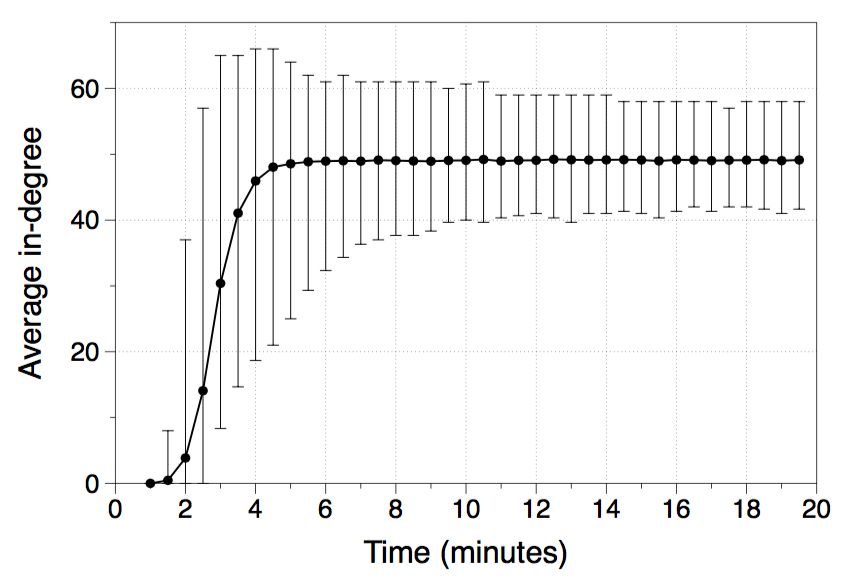
\includegraphics[keepaspectratio=true, width=1\linewidth]{images/paper_indegree_evolution}
  \caption{}
  \label{fig:paper_indegree_evolution}
\end{subfigure}
\caption{Measure of the in-degree evolution over time with error bars.~\ref{fig:indegree_evolution} represents our result,~\ref{fig:paper_indegree_evolution} is the test reported in the paper.}
\label{fig:randomness_indegree}
\end{figure}

Figure~\ref{fig:clustering_coefficient_evolution} shows the clustering coefficient evolution for different view size, as we can notice it grows with increasing the view size. In fact the higher the view, the higher the number of connections. This result is the same on the original paper. We can also notice that it converges roughly at the same rate as the in-degree.

\begin{figure}
\centering
\begin{subfigure}{.5\textwidth}
  \centering
  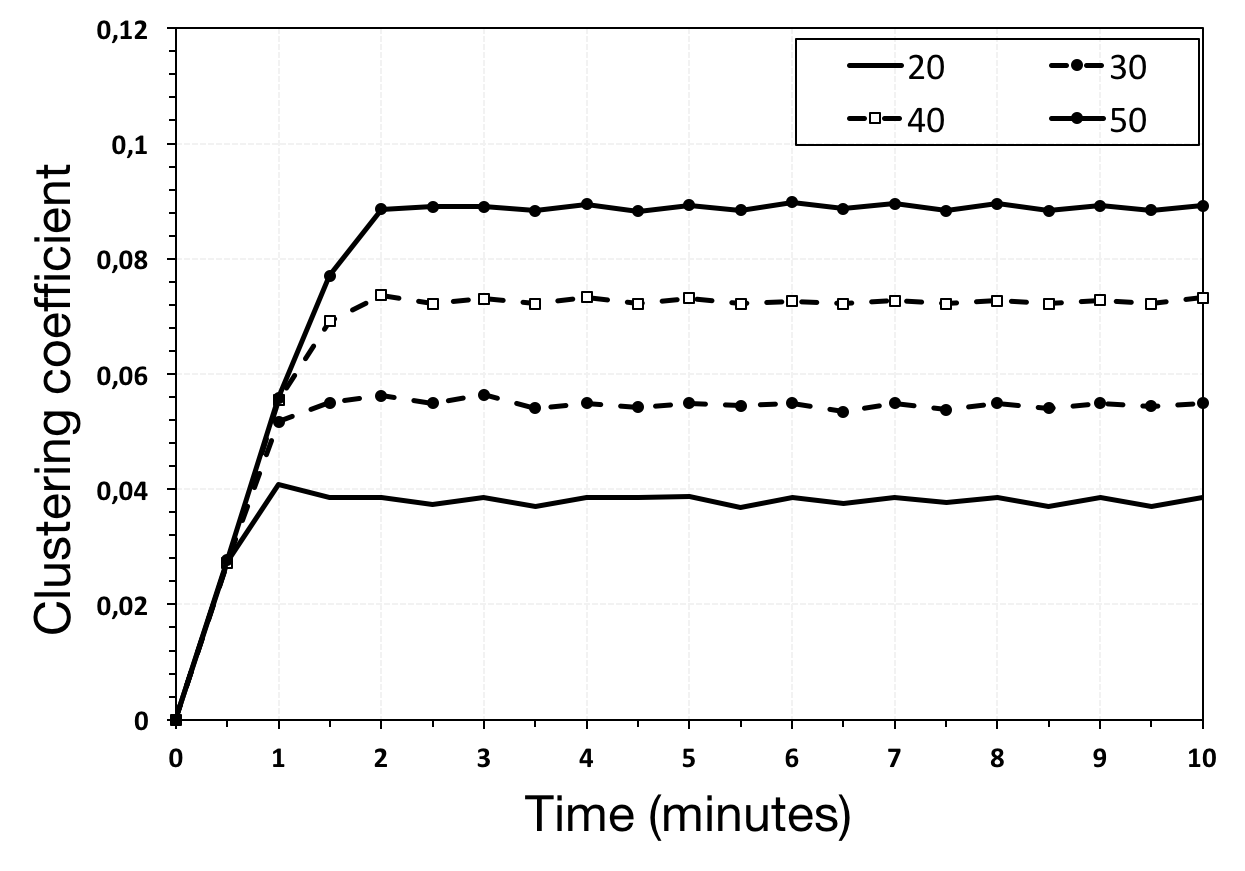
\includegraphics[keepaspectratio=true, width=1\linewidth]{images/clustering_coefficient_evolution}
  \caption{}
  \label{fig:clustering_coefficient_evolution}
\end{subfigure}%
\begin{subfigure}{.5\textwidth}
  \centering
  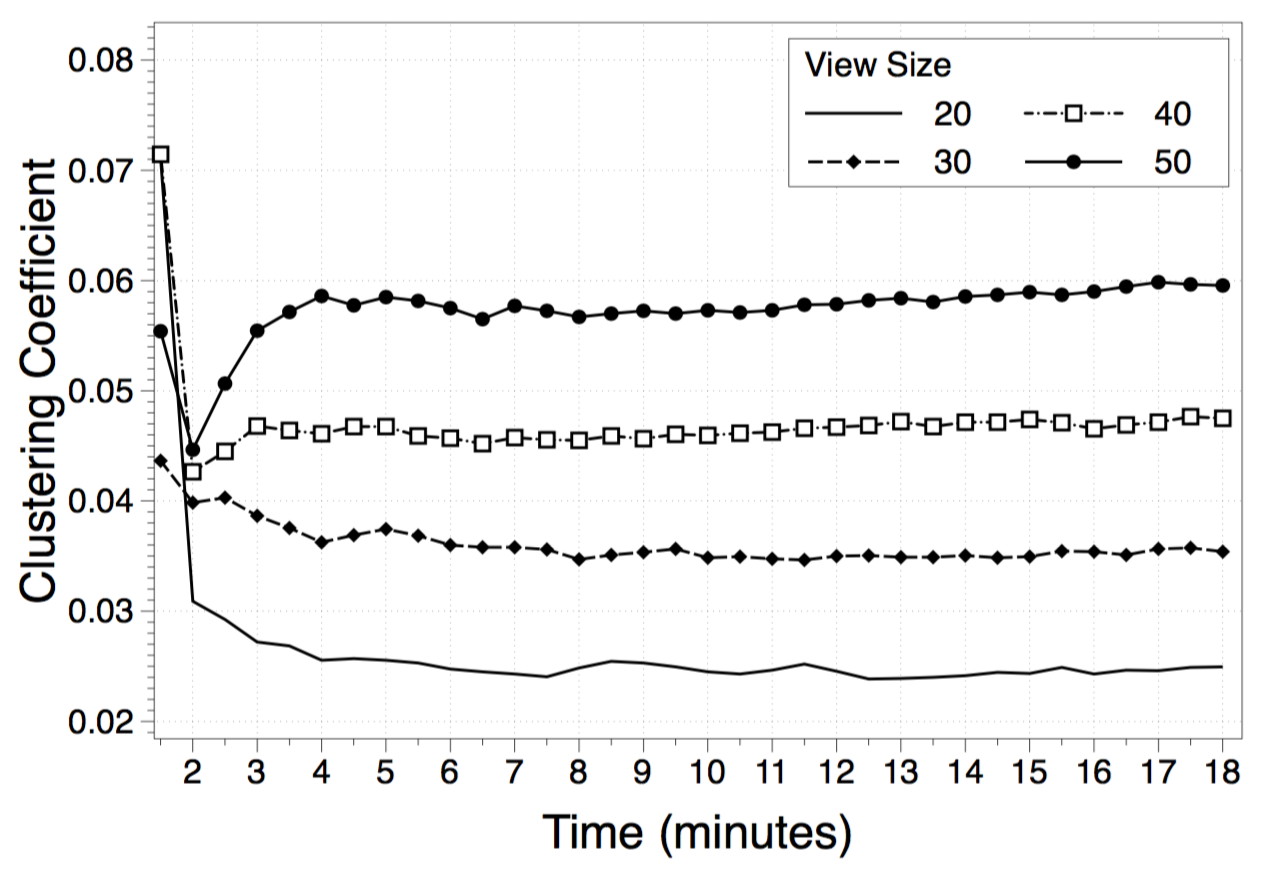
\includegraphics[keepaspectratio=true, width=1\linewidth]{images/paper_clustering_coefficient_evolution}
  \caption{}
  \label{fig:paper_clustering_coefficient_evolution}
\end{subfigure}
\caption{Clustering coefficient evolution over time with different view size.~\ref{fig:clustering_coefficient_evolution} represents our result,~\ref{fig:paper_clustering_coefficient_evolution} is the test reported in the paper.}
\label{fig:randomness_clustering}
\end{figure}

The last test is shown in Figure~\ref{fig:converged_clustering_coefficient} and it indicates that the clustering coefficient is higher than the one of the random graph by a constant factor, which is due to the fact that \ac{WPSS} does not guarantee independent samples at nodes that are close in the stable base overlay~\cite{wormhole}.

\begin{figure}
\centering
\begin{subfigure}{.5\textwidth}
  \centering
  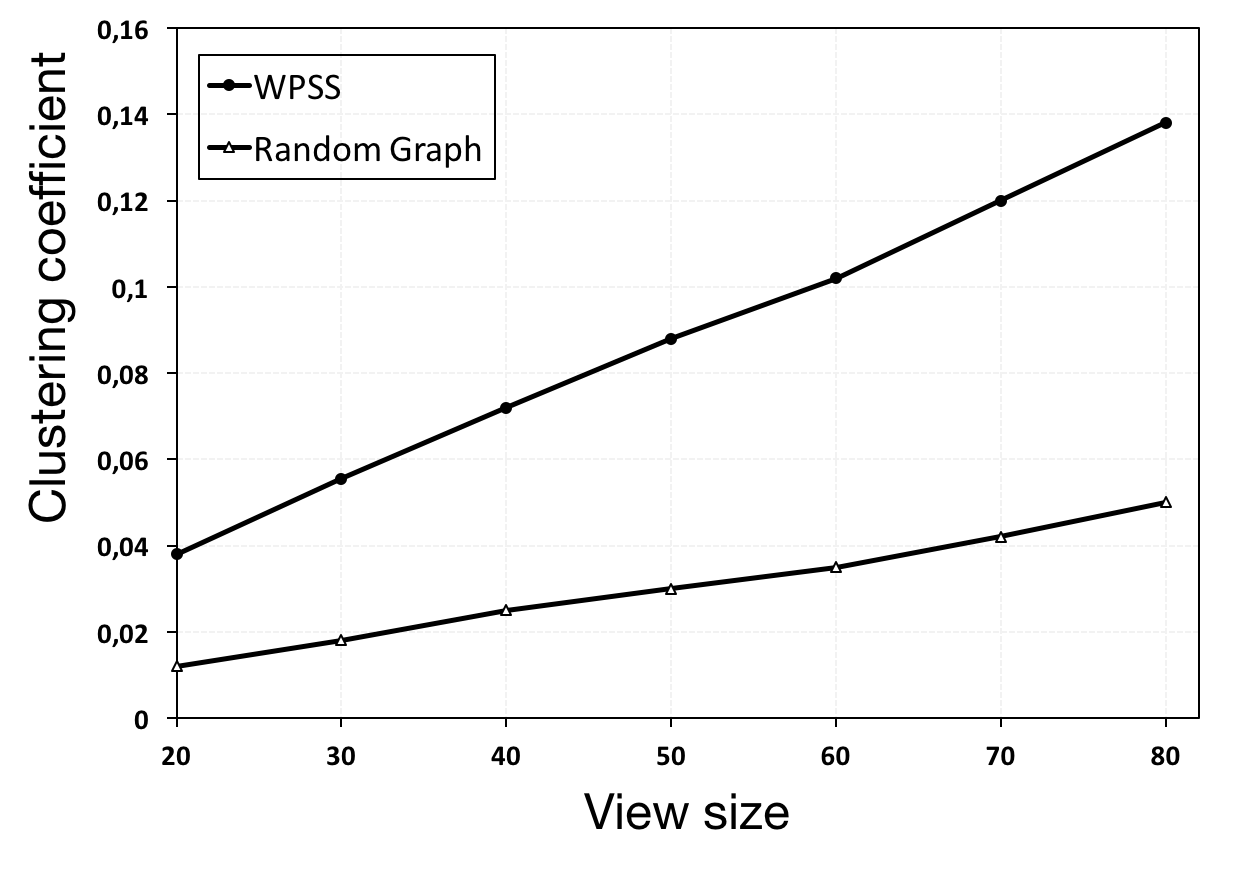
\includegraphics[keepaspectratio=true, width=1\linewidth]{images/converged_clustering_coefficient}
  \caption{}
  \label{fig:converged_clustering_coefficient}
\end{subfigure}%
\begin{subfigure}{.5\textwidth}
  \centering
  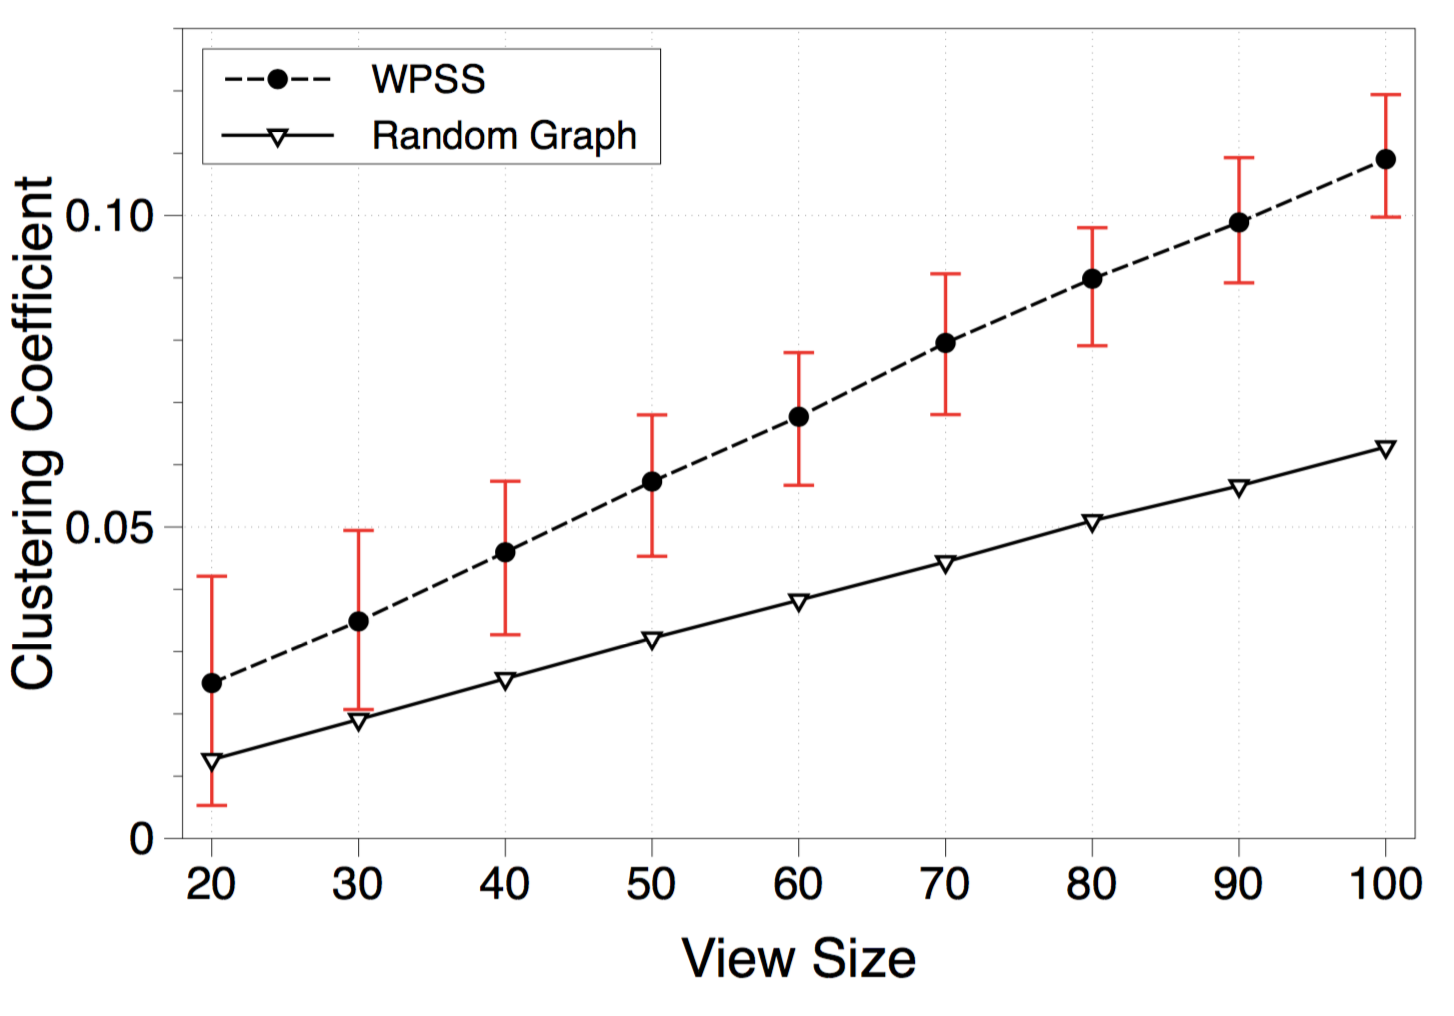
\includegraphics[keepaspectratio=true, width=1\linewidth]{images/paper_converged_clustering_coefficient}
  \caption{}
  \label{fig:paper_converged_clustering_coefficient}
\end{subfigure}
\caption{Converged clustering coefficient for increasing view sizes.~\ref{fig:converged_clustering_coefficient} represents our result,~\ref{fig:paper_converged_clustering_coefficient} is the test reported in the paper.}
\label{fig:randomness_conv_clustering}
\end{figure}

\newpage
\section{Inter-arrival Time of Advertisements}
\label{sec:interarrivaltime}
In these tests we want to measure the inter-arrival time of the advertisements, namely the lapse of time between two consecutive accepted samples. This is an important factor, because the topology is a constraint: in fact the public nodes have a lot of peers connected to them, so they receive more advertisements than the private nodes that instead have a lower number of connected peers. However, the \acceptAd method takes care of this: it ensures that all the nodes, in average, consume the advertisements at the same rate, namely one in each $\Delta$ period. In Figure~\ref{fig:average_interarrivaltime} we can observe that the average inter-arrival time of the samples converges to the wormhole period $\Delta$ after about 2 minutes. Except in this time lapse, all the nodes in average consume one advertisement every $\Delta$, which is exactly the result we were searching for. Furthermore, this result is identical to the one shown in the original paper.

\begin{figure}
\centering
\begin{subfigure}{.5\textwidth}
  \centering
  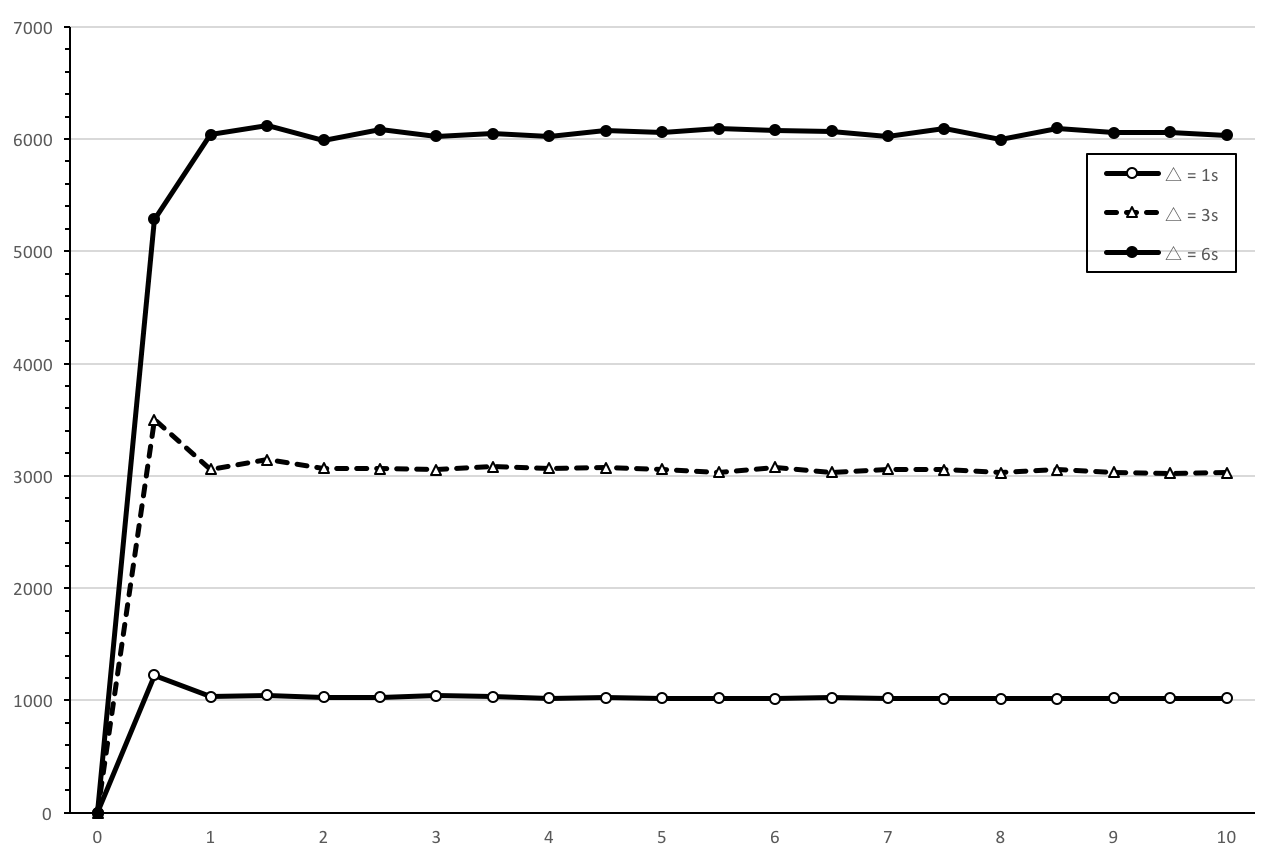
\includegraphics[keepaspectratio=true, width=1\linewidth]{images/average_interarrivaltime}
  \caption{}
  \label{fig:average_interarrivaltime}
\end{subfigure}%
\begin{subfigure}{.5\textwidth}
  \centering
  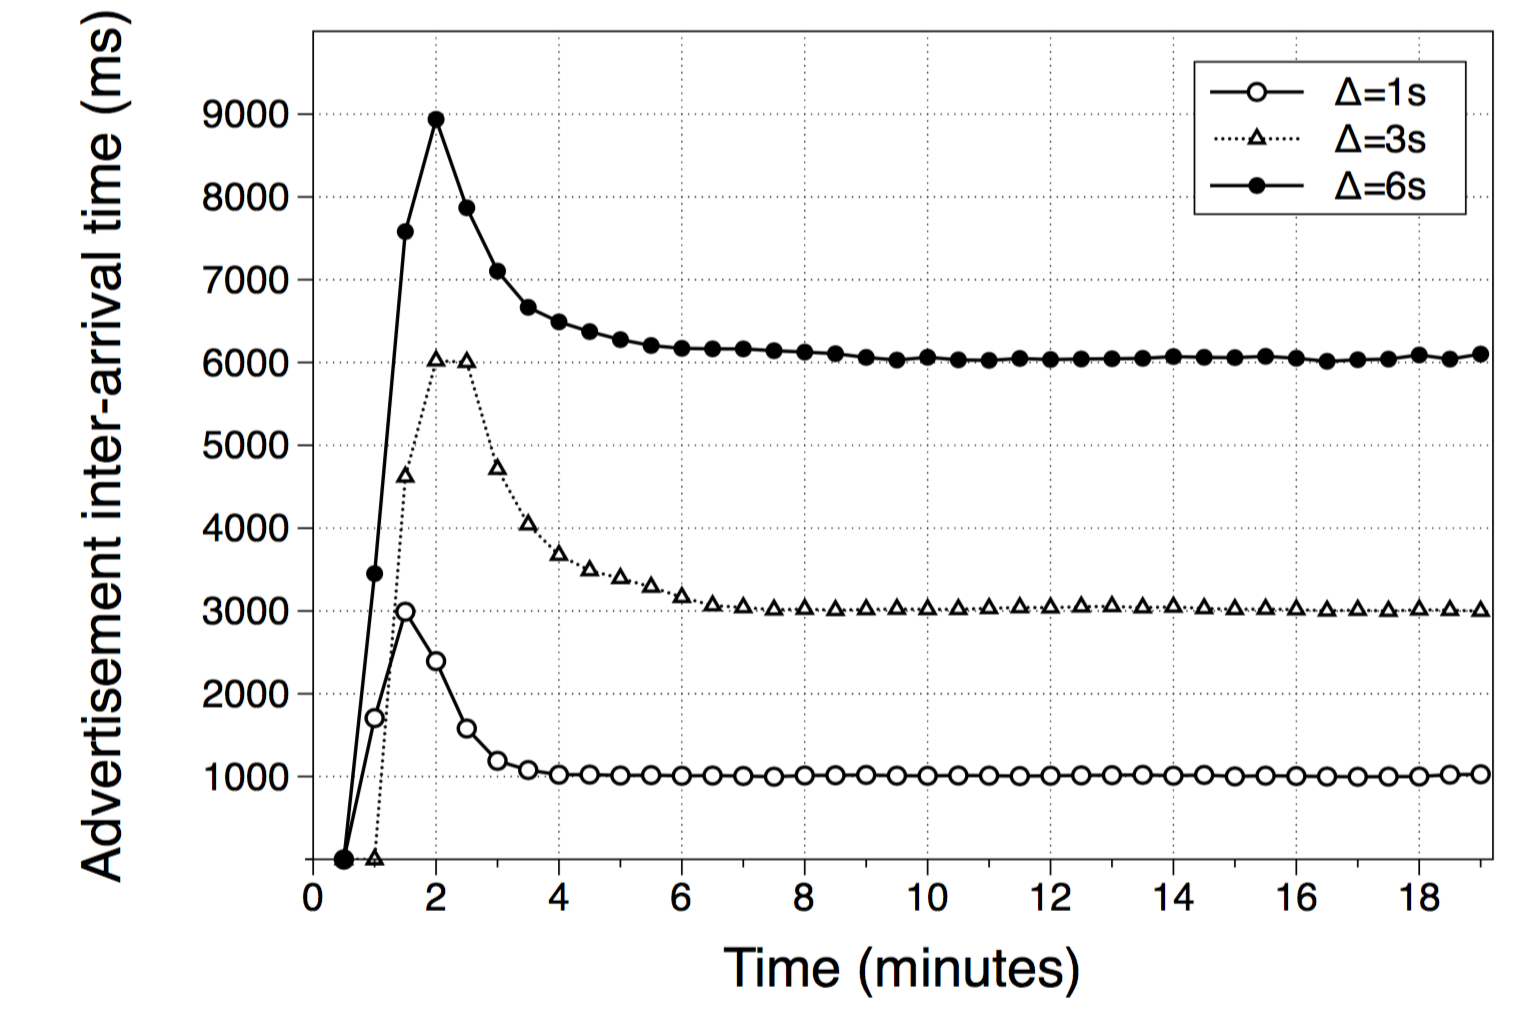
\includegraphics[keepaspectratio=true, width=1\linewidth]{images/paper_average_interarrivaltime}
  \caption{}
  \label{fig:paper_average_interarrivaltime}
\end{subfigure}
\caption{Average inter-arrival time for samples (terminating advertisements) at all peers.~\ref{fig:average_interarrivaltime} represents our result,~\ref{fig:paper_average_interarrivaltime} is the test reported in the paper.}
\label{fig:ad_average_interarrivaltime}
\end{figure}


Now we want to verify if the \acceptAd method correctly balances samples across public and private nodes. To do that, we measured the difference inter-arrival time between them. As shown in Figure~\ref{fig:interarrivaltime_difference} this difference is very low, about $500ms$ in the worst case in which $\Delta = 6 s$. With $\Delta$ equals to $1s$ or $3s$ the difference is lower, about $100ms$ and $200ms$, so we can confirm that the \acceptAd method successfully balances the samples between all the nodes, as well as in the original paper.

\begin{figure}
\centering
\begin{subfigure}{.5\textwidth}
  \centering
  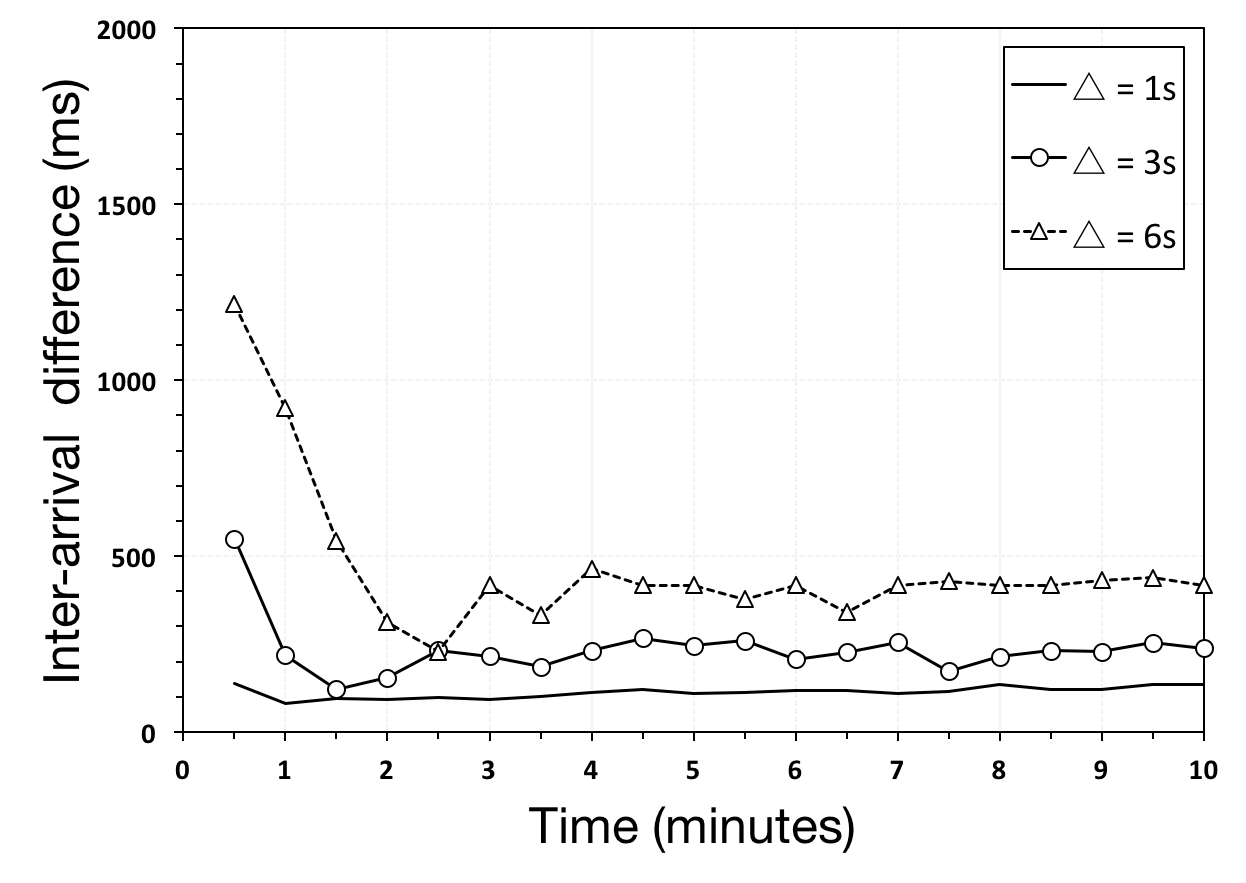
\includegraphics[keepaspectratio=true, width=1\linewidth]{images/interarrivaltime_difference}
  \caption{}
  \label{fig:interarrivaltime_difference}
\end{subfigure}%
\begin{subfigure}{.5\textwidth}
  \centering
  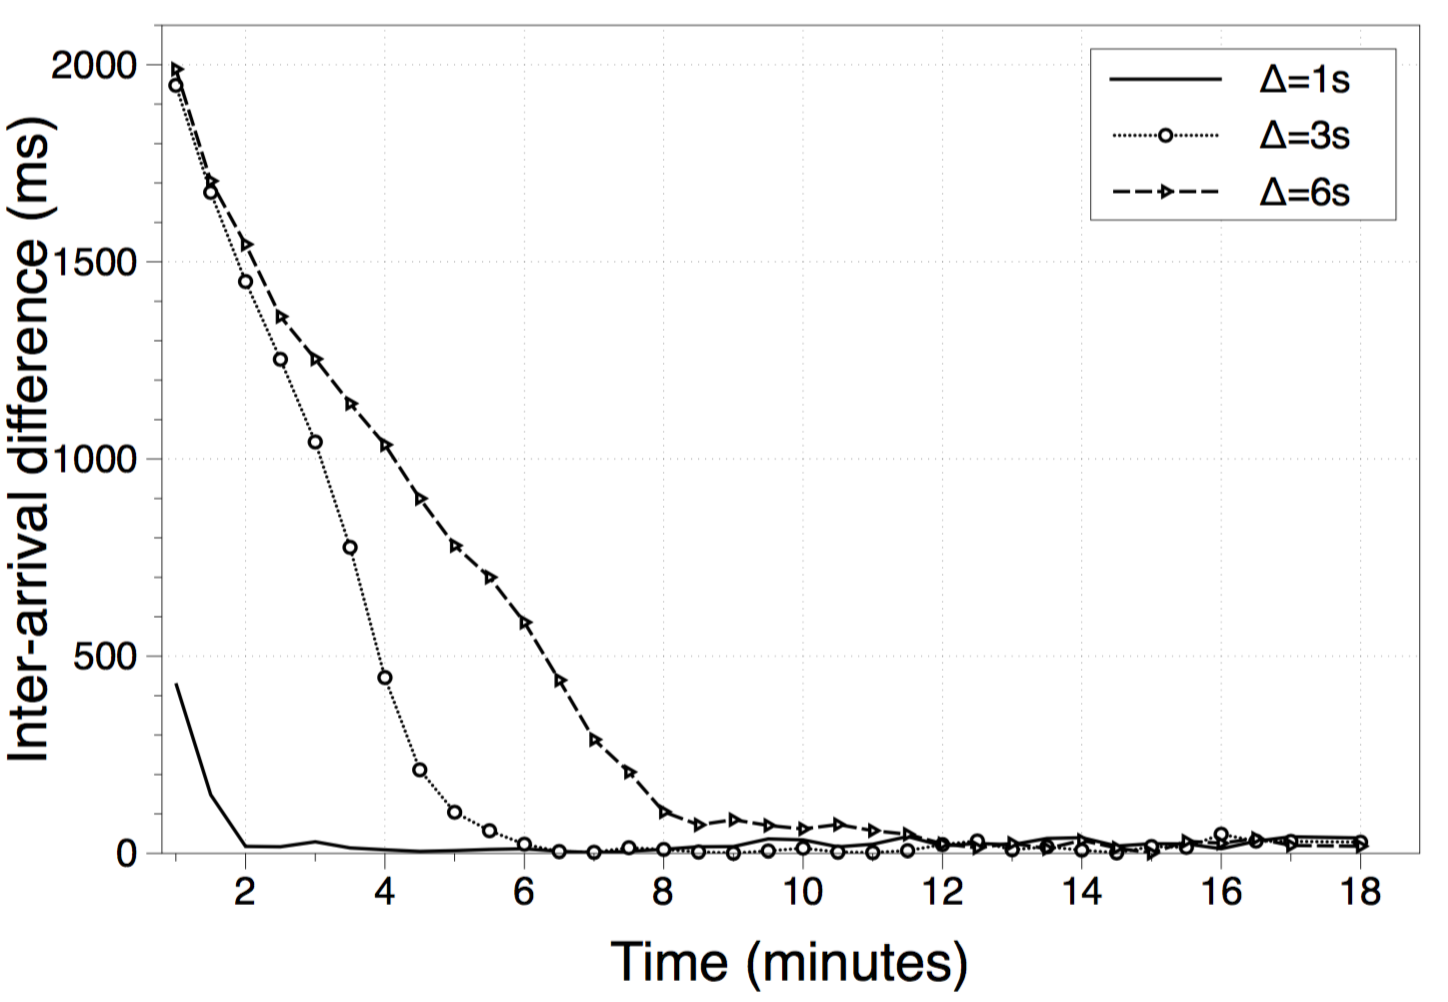
\includegraphics[keepaspectratio=true, width=1\linewidth]{images/paper_interarrivaltime_difference}
  \caption{}
  \label{fig:paper_interarrivaltime_difference}
\end{subfigure}
\caption{Difference in inter-arrival time between public and private peers.~\ref{fig:interarrivaltime_difference} represents our result,~\ref{fig:paper_interarrivaltime_difference} is the test reported in the paper.}
\label{fig:ad_interarrivaltime_difference}
\end{figure}


\section{Robustness to Different Churn Patterns}
\label{sec:robustness}
In this set of experiments we want to test the robustness of our implementation under different levels of churn. We measure the average hop count, as well as the clustering coefficient and the in-degree. For the experiments related to the average hop count, we test also the two versions of the \getMetropolisHastingsNeighbour function: when we call it over all the connected peers or, as in the original paper, over the base overlay.

In the first three experiments we recreate a flash crowd scenario, in which some nodes join at the beginning and the remaining ones join at a later point in time. For instance, recalling that $N = 1000$, for a flash crowd scenario of 70\% of the node, 300 nodes join at time $0s$ and 700 nodes join at minute 6.5. Then after this time, the number of nodes remains constant at 1000. 

In Figure~\ref{fig:average_hop_count_flash_crowd_1impl} we can see that the average hop count increases with decreasing the number of nodes that join the system at time 0, in fact an advertisement will have to traverse more nodes in order to reach a peer that does not already have that sample. However at time 7, when all the remaining nodes join the system, the average hop count not only stabilizes quickly, but it converges to the same value in all the experiments. In Figure~\ref{fig:average_hop_count_flash_crowd_2impl} there is the second implementation, as expected the average hop count is a little bit higher, however it still converges to the same value at time 7. In Figure~\ref{fig:paper_average_hop_count_flash_crowd} instead is shown their result and as we can see they are almost identical, as expected it stabilizes at the same rate as in our second implementation. 

\begin{figure}
\centering
\begin{subfigure}{.5\textwidth}
  \centering
  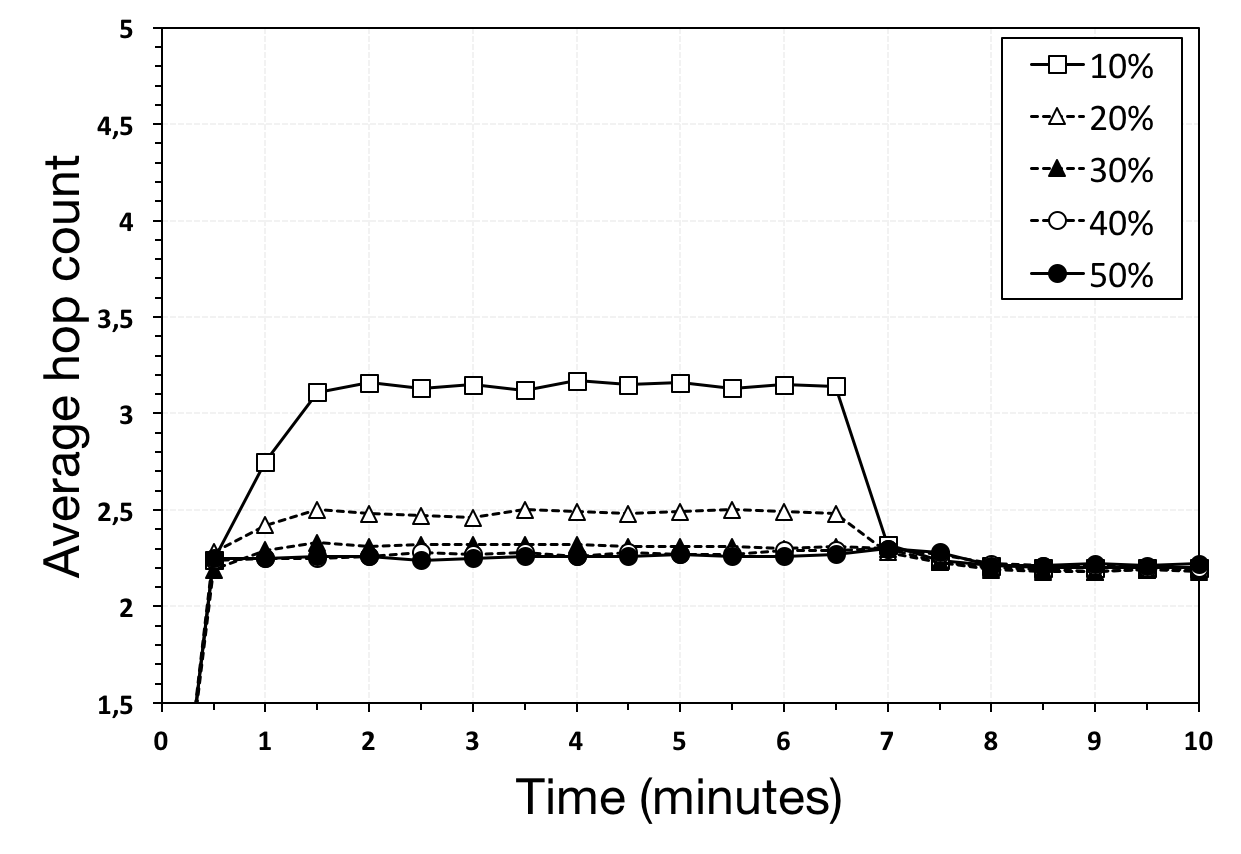
\includegraphics[keepaspectratio=true, width=1\linewidth]{images/average_hop_count_flash_crowd_1impl}
  \caption{}
  \label{fig:average_hop_count_flash_crowd_1impl}
\end{subfigure}%
\begin{subfigure}{.5\textwidth}
  \centering
  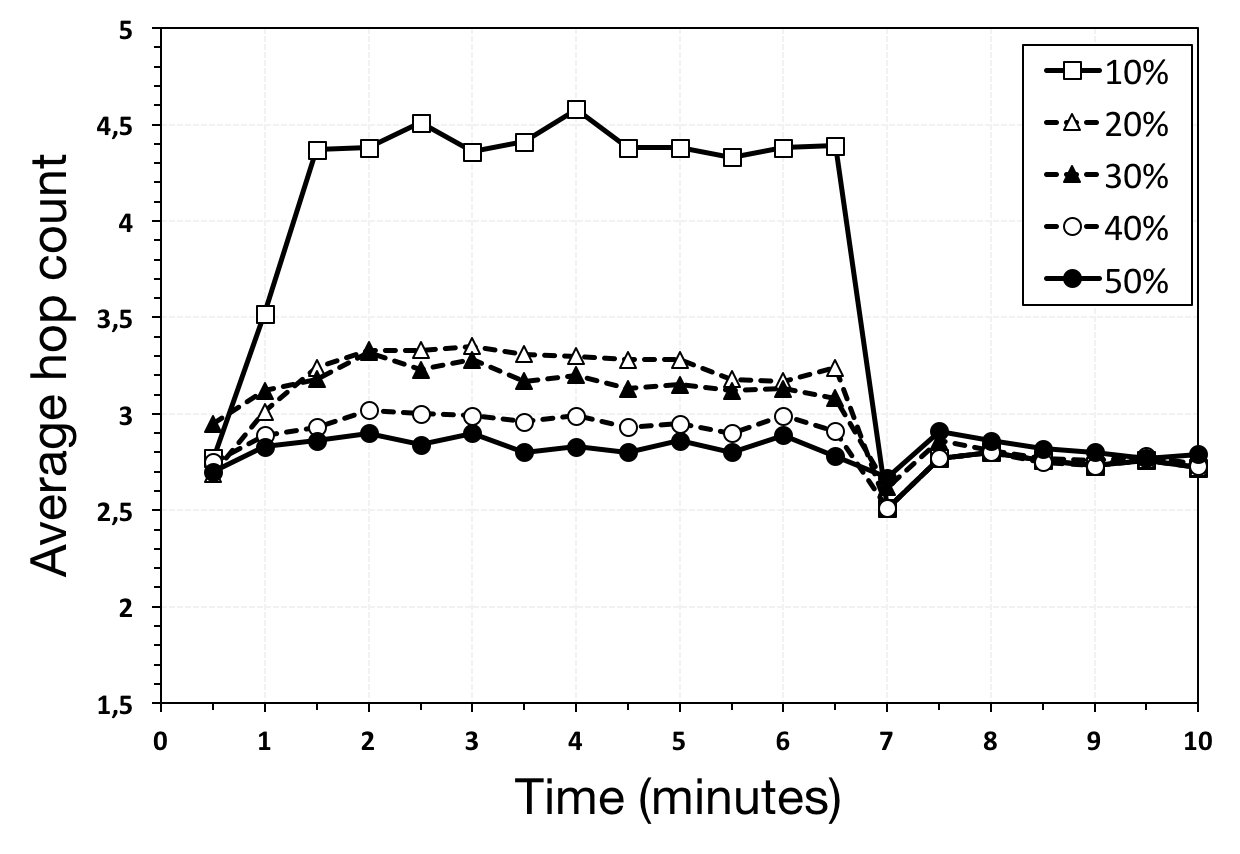
\includegraphics[keepaspectratio=true, width=1\linewidth]{images/average_hop_count_flash_crowd_2impl}
  \caption{}
  \label{fig:average_hop_count_flash_crowd_2impl}
\end{subfigure}
\begin{subfigure}{.5\textwidth}
  \centering
  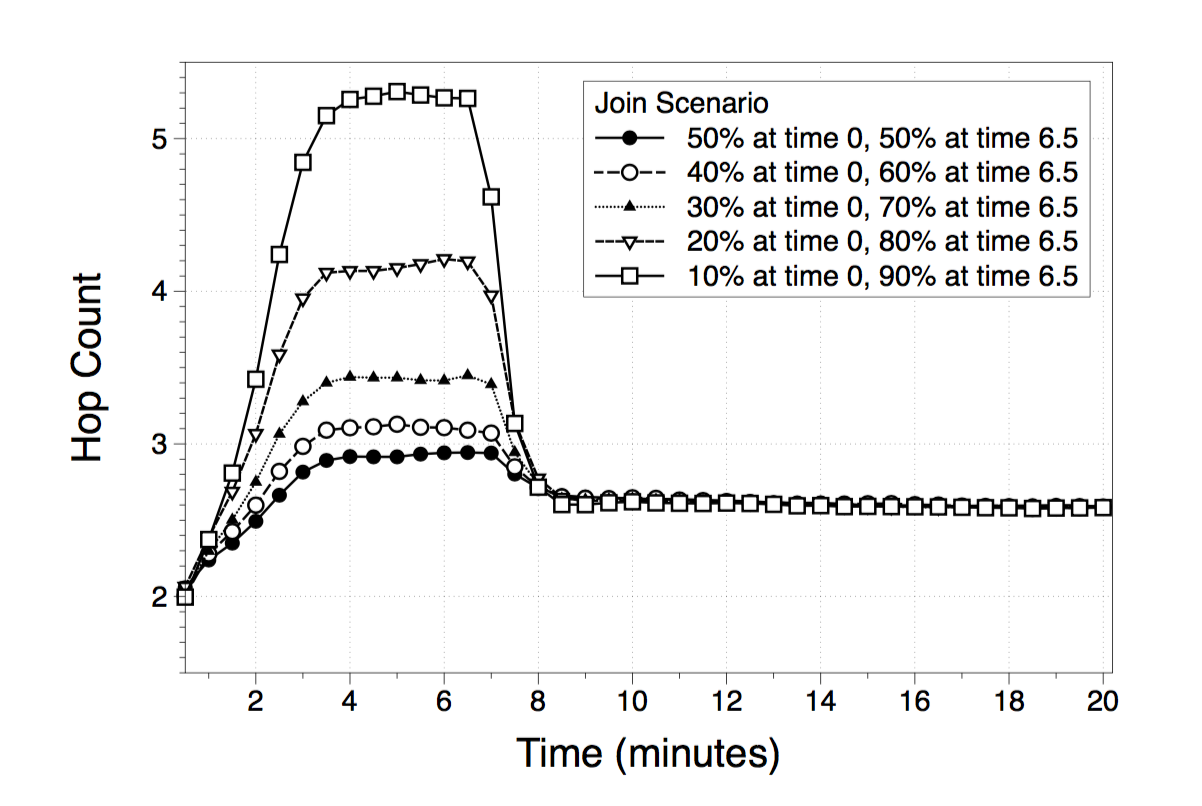
\includegraphics[keepaspectratio=true, width=1\linewidth]{images/paper_average_hop_count_flash_crowd}
  \caption{}
  \label{fig:paper_average_hop_count_flash_crowd}
\end{subfigure}
\caption{Average hop count in a flash crowd scenario.~\ref{fig:average_hop_count_flash_crowd_1impl} represents our result in the first implementation (\getMetropolisHastingsNeighbour over all the connected peers),~\ref{fig:average_hop_count_flash_crowd_2impl} represent our result in the second implementation(\getMetropolisHastingsNeighbour over the base overlay) and~\ref{fig:paper_average_hop_count_flash_crowd} is the test reported in the paper.}
\label{fig:robustness_hop_count_flash_crowd}
\end{figure}

The next test measures the clustering coefficient in a flash crowd scenario, the expected behaviour is similar to the average hop count. As shown in Figure~\ref{fig:average_clustering_coefficient_flash_crowd}, this is the case, in fact the clustering coefficient stabilizes quickly and to the same rate when all the nodes join the network. Figure~\ref{fig:paper_average_clustering_coefficient_flash_crowd} shows their result, our clustering coefficient is a little bit higher compared to this, however it could derive from the fact that in order to establish new connections we use a tracker instead of random walks.

\begin{figure}
\centering
\begin{subfigure}{.5\textwidth}
  \centering
  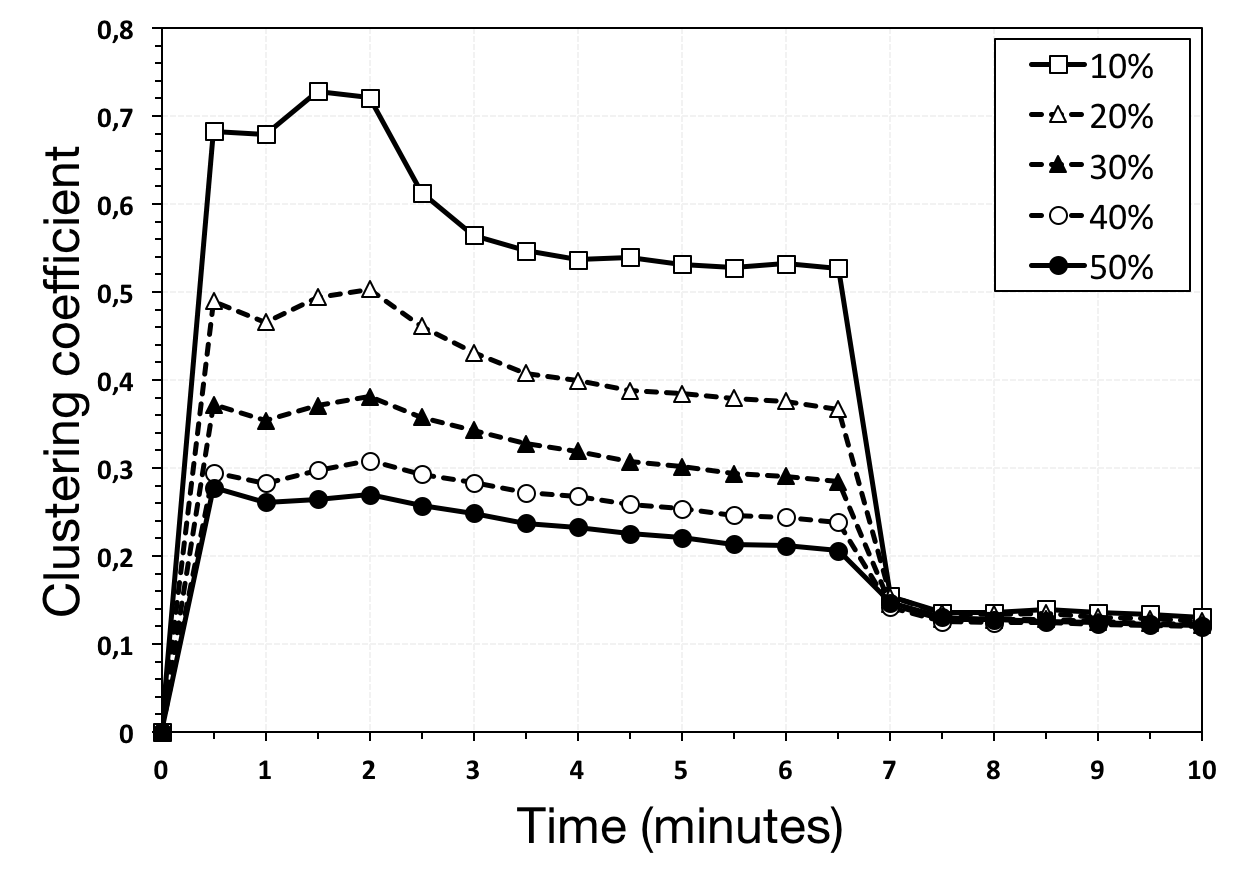
\includegraphics[keepaspectratio=true, width=1\linewidth]{images/average_clustering_coefficient_flash_crowd}
  \caption{}
  \label{fig:average_clustering_coefficient_flash_crowd}
\end{subfigure}%
\begin{subfigure}{.5\textwidth}
  \centering
  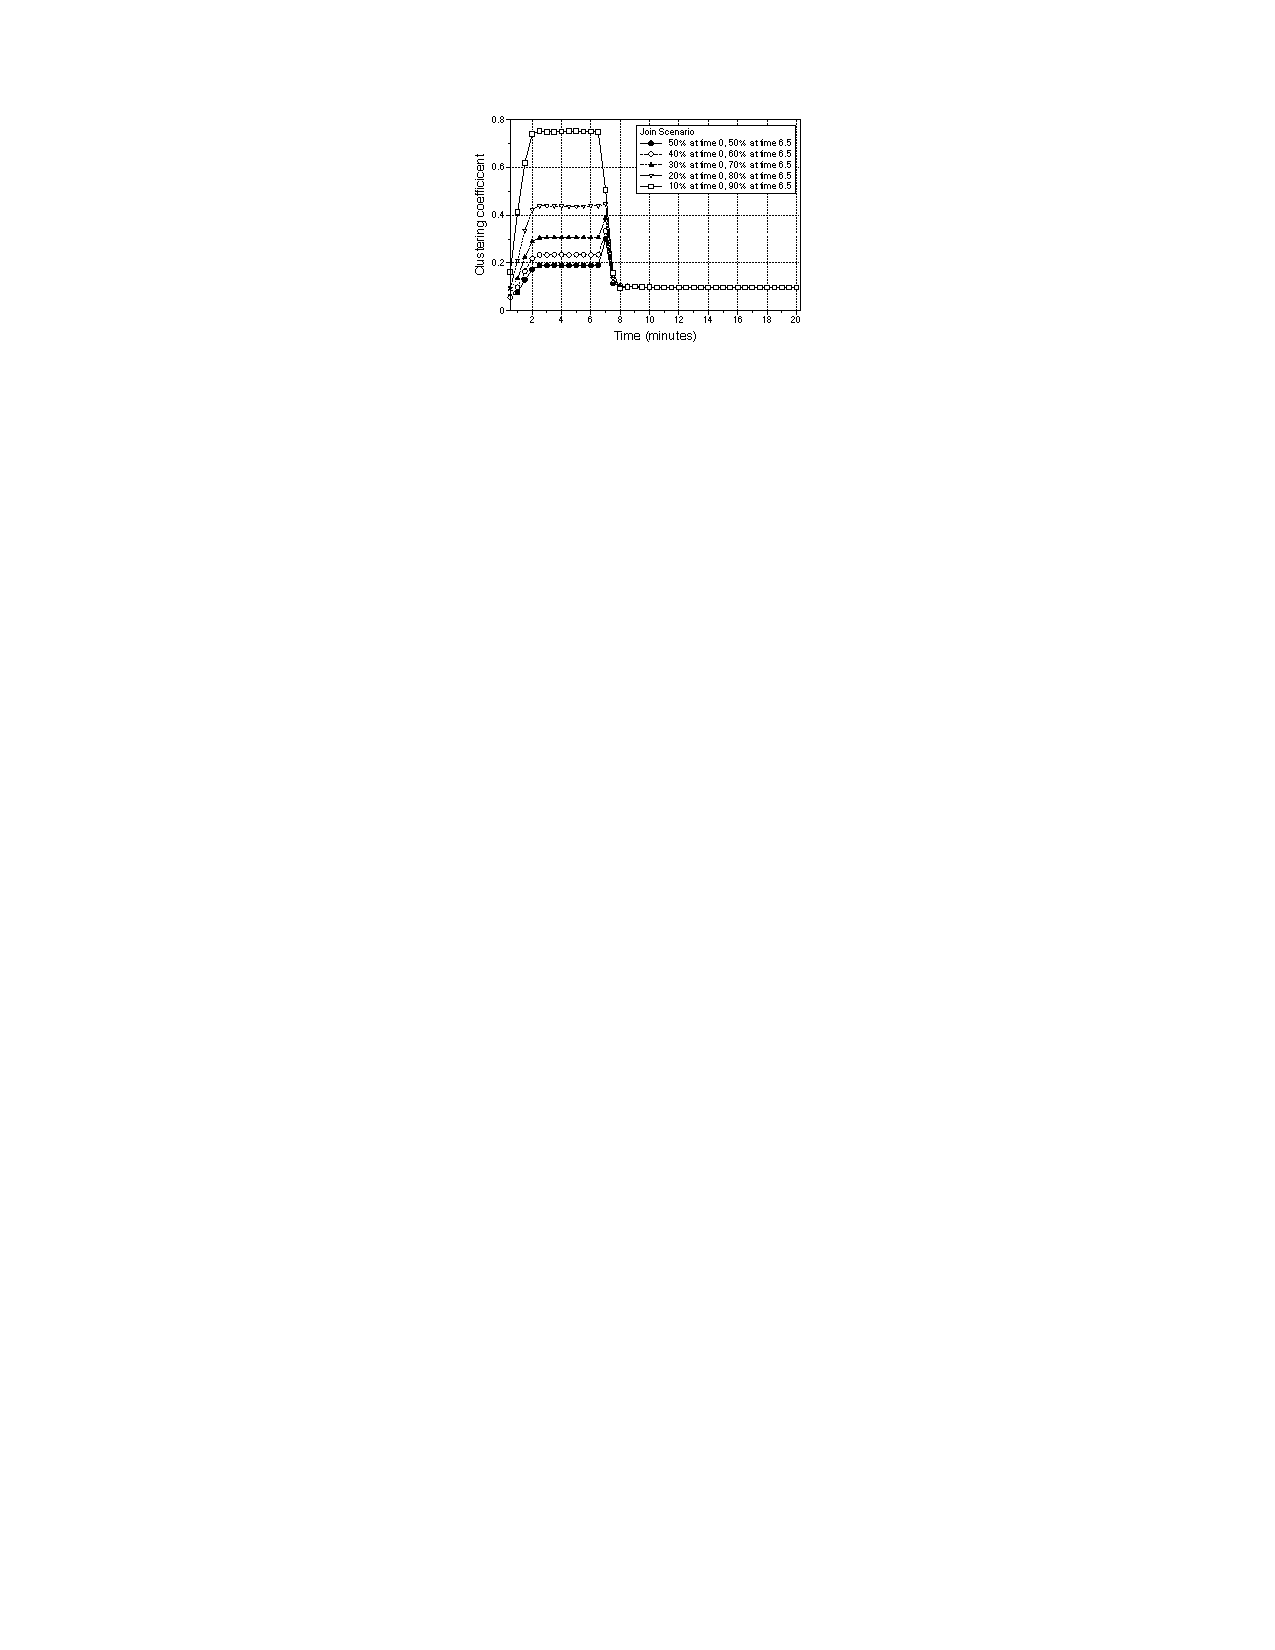
\includegraphics[keepaspectratio=true, width=1\linewidth]{images/paper_average_clustering_coefficient_flash_crowd}
  \caption{}
  \label{fig:paper_average_clustering_coefficient_flash_crowd}
\end{subfigure}
\caption{Clustering coefficient evolution in a flash crowd scenario.~\ref{fig:average_clustering_coefficient_flash_crowd} represents our result,~\ref{fig:paper_average_clustering_coefficient_flash_crowd} is the test reported in the paper.}
\label{fig:robustness_cc_flash_crowd}
\end{figure}

Finally, Figure~\ref{fig:average_indegree} shows the average in-degree of the nodes. As we can see after two minutes in all the experiments the nodes have in average the same in-degree, then it drops significantly at time 6.5, this is in fact expected since a majority of nodes join the network with in-degree equals to 0. However, it recovers quickly (about 1.30 minutes later) and it converges to 50 in all the experiments. Figure~\ref{fig:paper_average_indegree} shows their result, as we can notice we obtained the same result.

\begin{figure}
\centering
\begin{subfigure}{.5\textwidth}
  \centering
  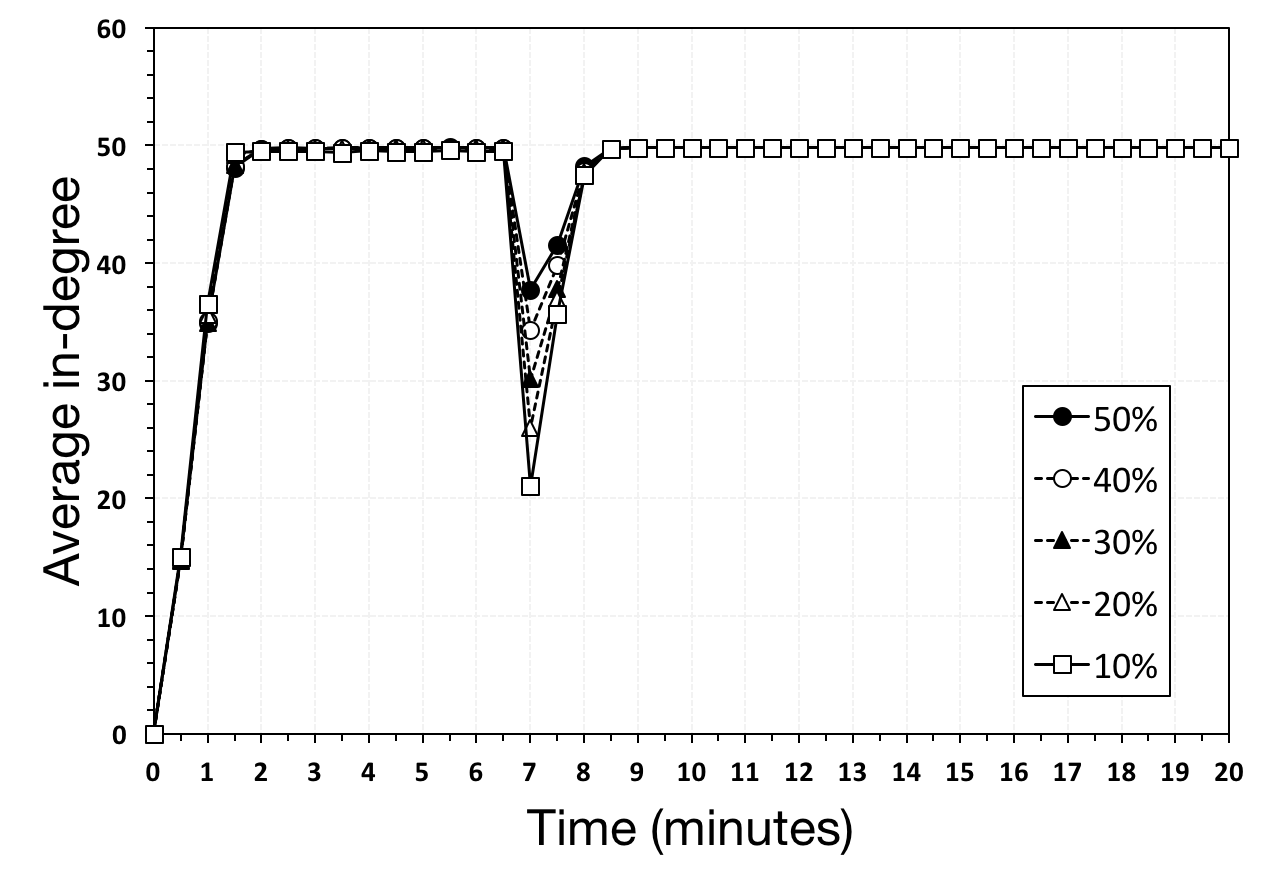
\includegraphics[keepaspectratio=true, width=1\linewidth]{images/average_indegree}
  \caption{}
  \label{fig:average_indegree}
\end{subfigure}%
\begin{subfigure}{.5\textwidth}
  \centering
  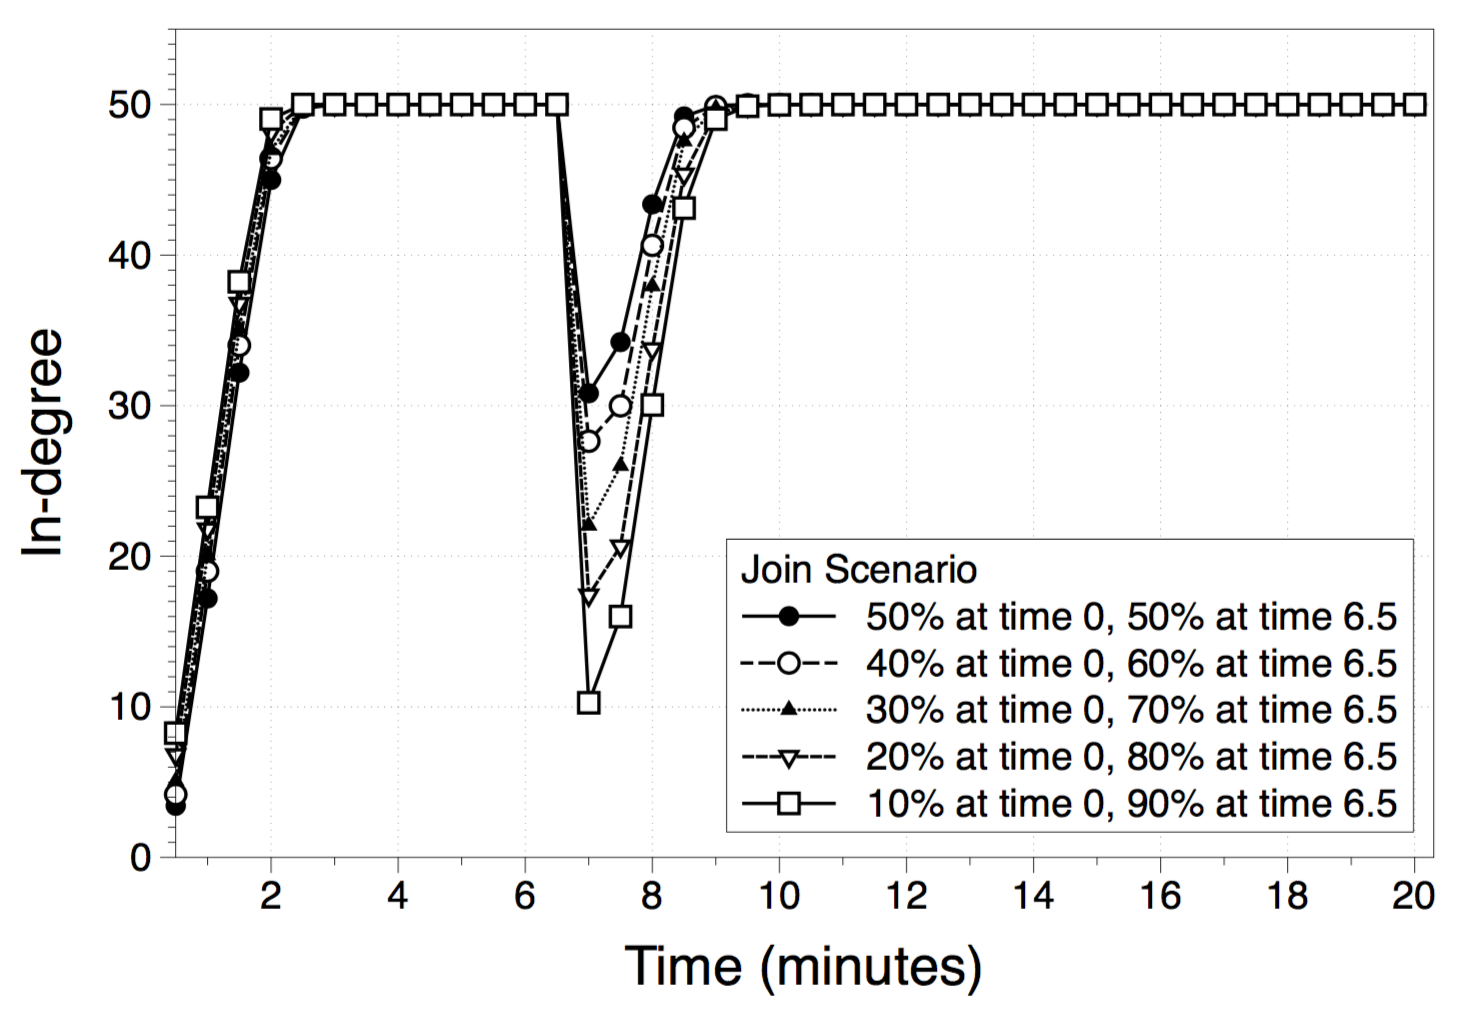
\includegraphics[keepaspectratio=true, width=1\linewidth]{images/paper_average_indegree}
  \caption{}
  \label{fig:paper_average_indegree}
\end{subfigure}
\caption{Average in-degree in a flash crowd scenario.~\ref{fig:average_indegree} represents our result,~\ref{fig:paper_average_indegree} is the test reported in the paper.}
\label{fig:robustness_indegree_flash_crowd}
\end{figure}

\newpage
In the next set of experiments we measure the robustness of our implementation in case of catastrophic failures, that is, when a large number of peers leave the system at a single instant in time. All the nodes join the system at time 0, we wait for the overlay to stabilize and then we fail a fixed percentage of nodes at time 5 minutes. We expect that the algorithm recovers quickly and also that all the nodes remain connected, even in the worst case scenario where 80\% of the peers leave the system. As in the previous set of experiments, we test both the implementation of the \getMetropolisHastingsNeighbour.

In Figure~\ref{fig:average_hop_count_failures_1impl} we can notice that all the experiments have the same average hop count until minute 5, then it increases with the increasing of failures. This is expected given the large number of broken links to detect and repair for both the base and wormhole overlays. Notice that the network remains connected even when 80\% of the nodes fail. Figure~\ref{fig:average_hop_count_failures_2impl} shows the second implementation, as expected the average hop count, compared to the first implementation, is a little bit higher after the mass failure. Figure~\ref{fig:paper_average_hop_count_failures} instead shows the result reported in the paper, as we can notice they have a quite bigger average hop count than us, which is probably due to the different implementations of the tracker and random walks.

\begin{figure}
\centering
\begin{subfigure}{.5\textwidth}
  \centering
  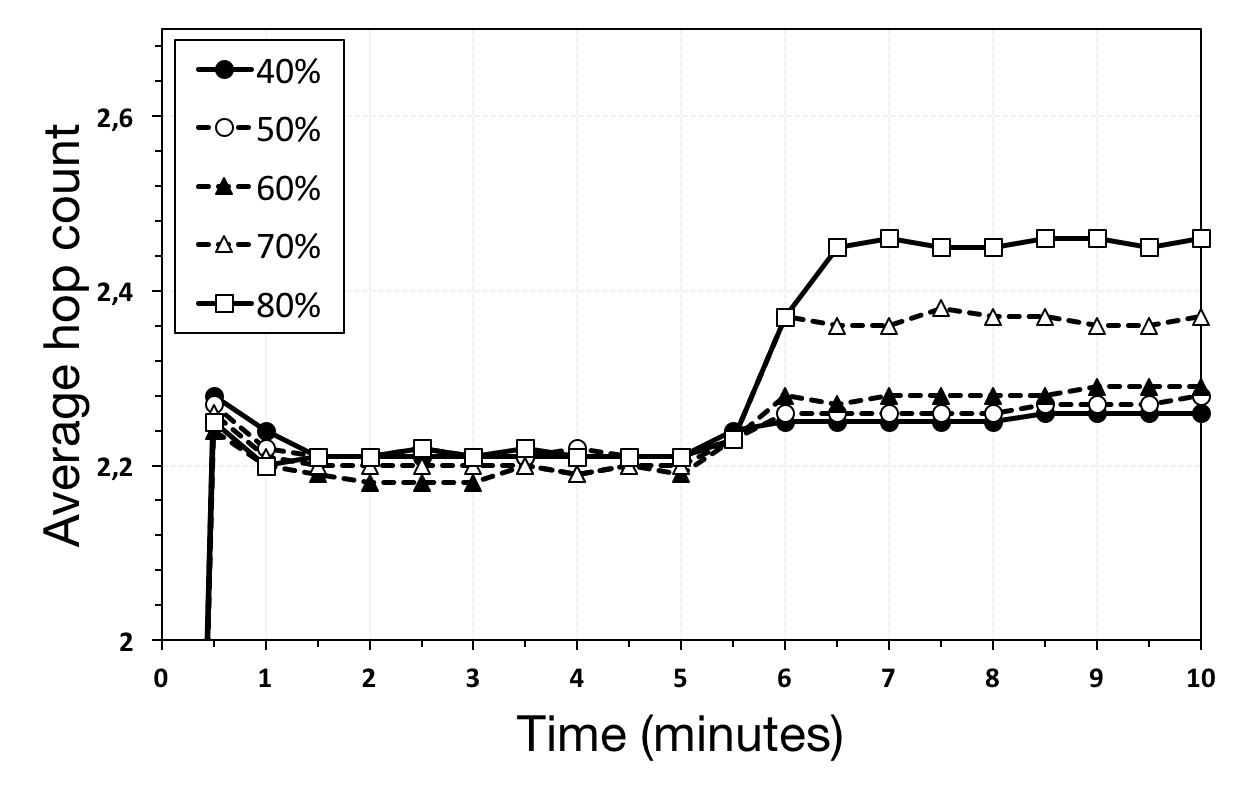
\includegraphics[keepaspectratio=true, width=1\linewidth]{images/average_hop_count_failures_1impl}
  \caption{}
  \label{fig:average_hop_count_failures_1impl}
\end{subfigure}%
\begin{subfigure}{.5\textwidth}
  \centering
  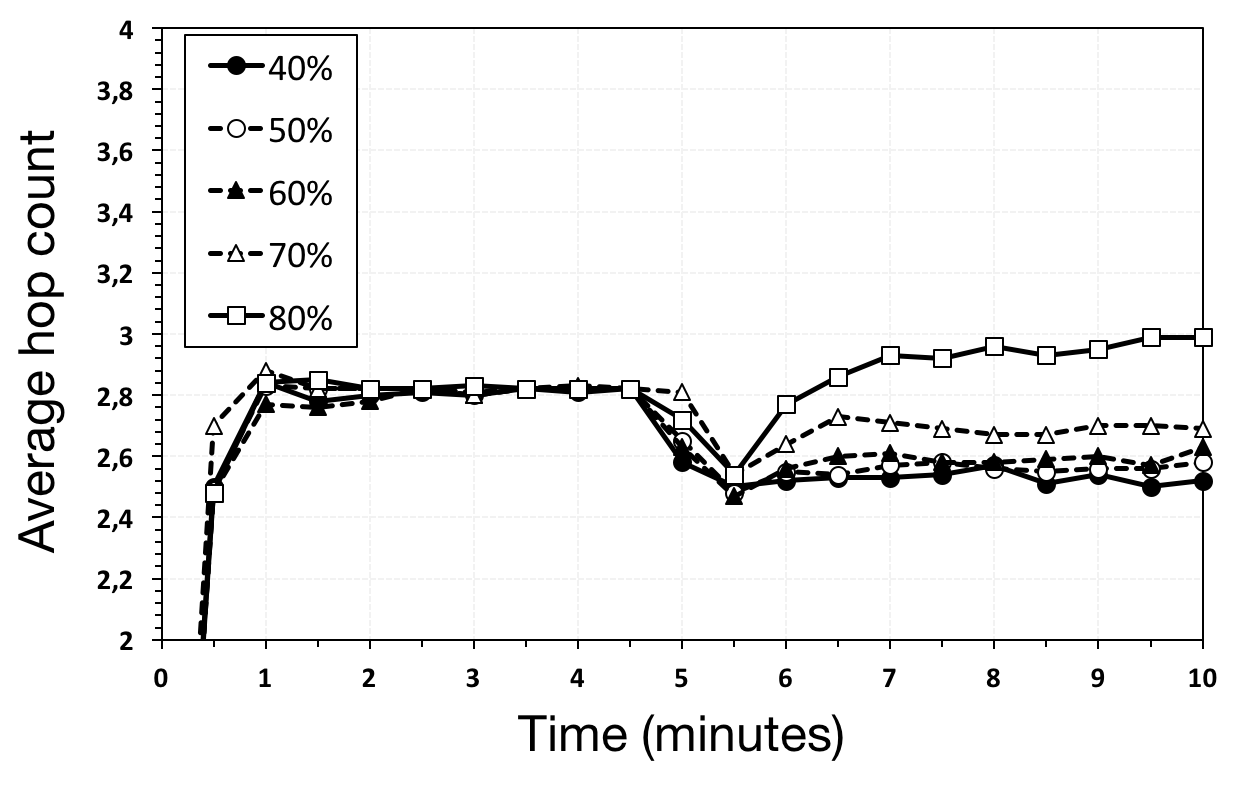
\includegraphics[keepaspectratio=true, width=1\linewidth]{images/average_hop_count_failures_2impl}
  \caption{}
  \label{fig:average_hop_count_failures_2impl}
\end{subfigure}
\begin{subfigure}{.5\textwidth}
  \centering
  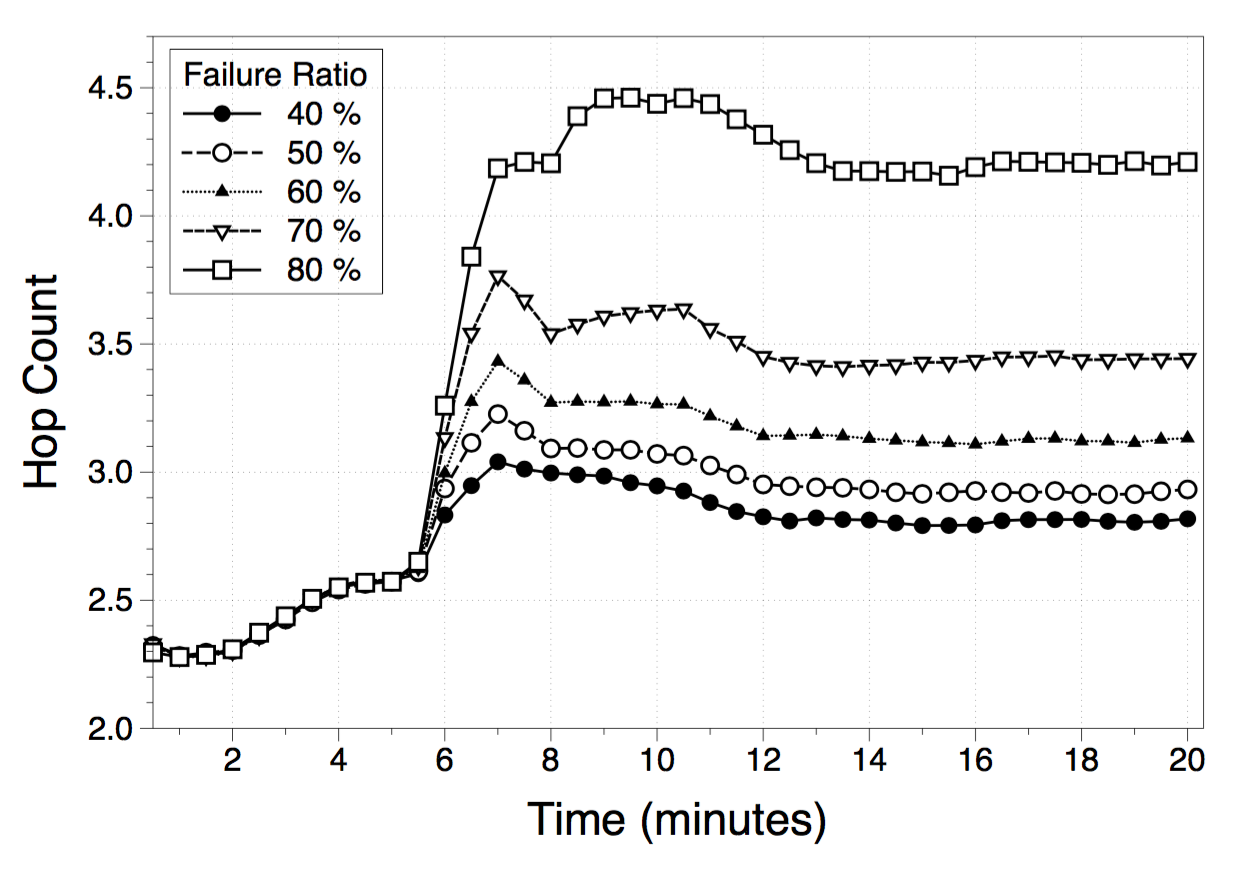
\includegraphics[keepaspectratio=true, width=1\linewidth]{images/paper_average_hop_count_failures}
  \caption{}
  \label{fig:paper_average_hop_count_failures}
\end{subfigure}
\caption{Average hop count in catastrophic failure scenarios with different ratios of failed nodes. ~\ref{fig:average_hop_count_failures_1impl} represents our result in the first implementation (\getMetropolisHastingsNeighbour over all the connected peers),~\ref{fig:average_hop_count_failures_2impl} represent our result in the second implementation(\getMetropolisHastingsNeighbour over the base overlay) and~\ref{fig:paper_average_hop_count_failures} is the test reported in the paper.}
\label{fig:robustness_hop_count_failures}
\end{figure}

Figure~\ref{fig:average_clustering_coefficient_failures} shows the evolution of the clustering coefficient: it increases with the increasing of failures, since there are less nodes in the network and they are much more connected between each other. 

\begin{figure}
\centering
\begin{subfigure}{.5\textwidth}
  \centering
  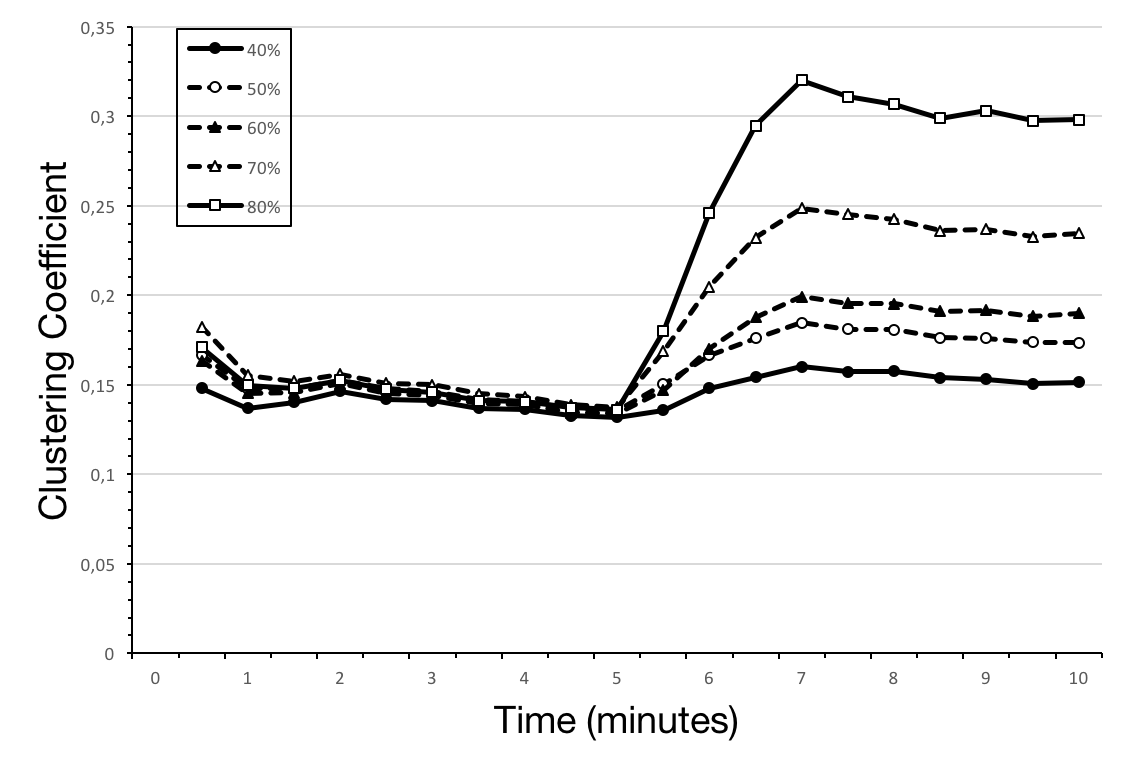
\includegraphics[keepaspectratio=true, width=1\linewidth]{images/average_clustering_coefficient_failures}
  \caption{}
  \label{fig:average_clustering_coefficient_failures}
\end{subfigure}%
\begin{subfigure}{.5\textwidth}
  \centering
  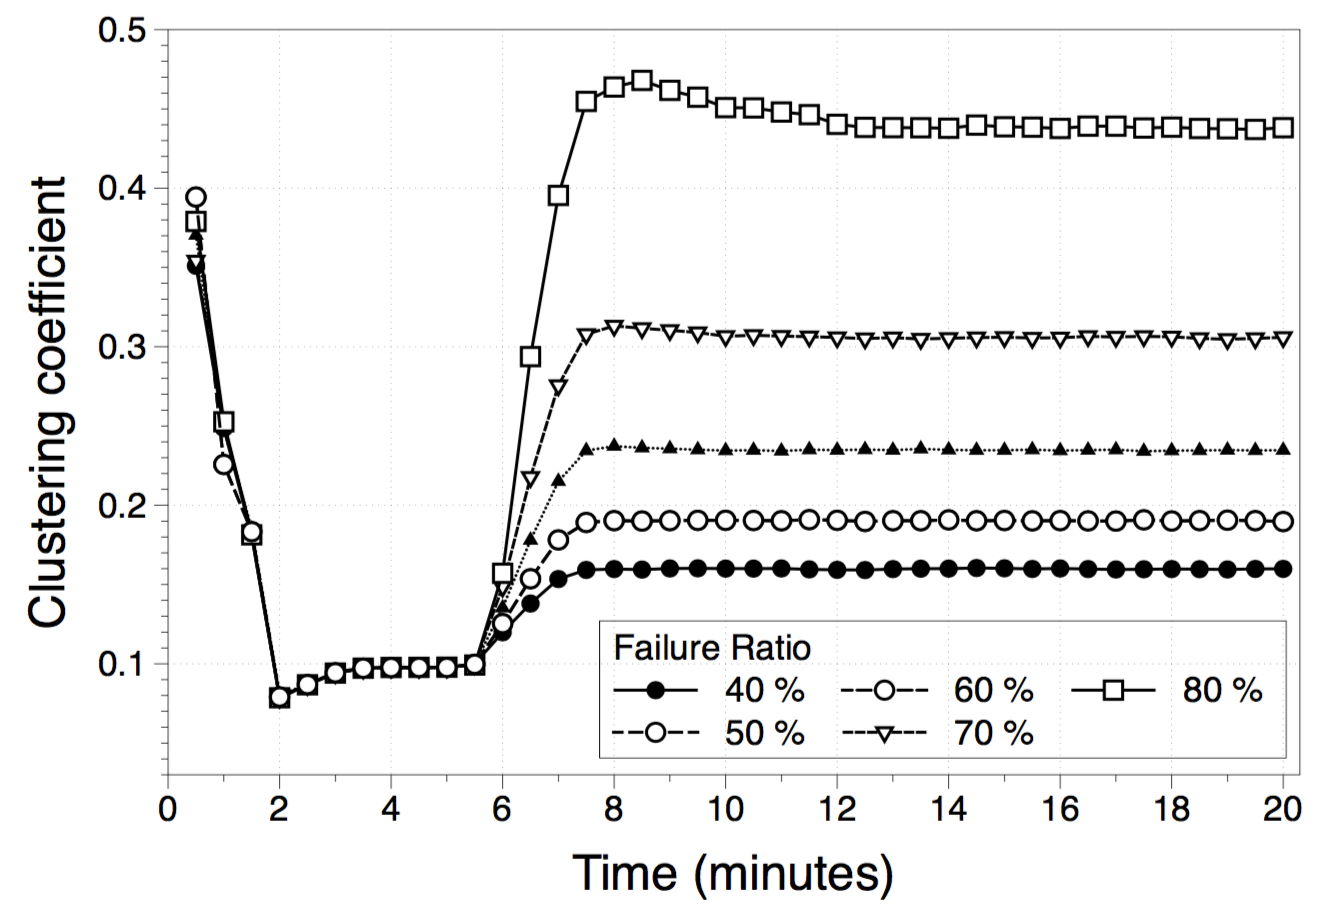
\includegraphics[keepaspectratio=true, width=1\linewidth]{images/paper_average_clustering_coefficient_failures}
  \caption{}
  \label{fig:paper_average_clustering_coefficient_failures}
\end{subfigure}
\caption{Clustering coefficient evolution in a flash crowd scenario.~\ref{fig:average_clustering_coefficient_failures} represents our result,~\ref{fig:paper_average_clustering_coefficient_failures} is the test reported in the paper.}
\label{fig:robustness_clustering_coefficient_failures}
\end{figure}

One important experiment in case of massive failures is to measure the average number of dead links in the views of the peers. What we want to obtain is a system which detect and replace the broken links as fast as possible, and in the same way it has to eliminate all the dead links from the views of the live nodes. Figure~\ref{fig:average_dead_links} shows the result: at time 5 the number of dead links increases (obviously the higher the failures, the higher the number of dead links), but anyway after just one minute all the broken links are successfully deleted from the views (even in the worst case where 80\% of the nodes fail), and the average number returns equal to zero. This result is even better than the one shown in the original paper, because the time employed by them to replace the links is two minutes, while our system takes half the time to do it. This is probably due the fact that we use a tracker, which has high availability and it responds to all the nodes immediately, while they use random walks, so they need more time to find a node and establish a new network connection.

\begin{figure}
\centering
\begin{subfigure}{.5\textwidth}
  \centering
  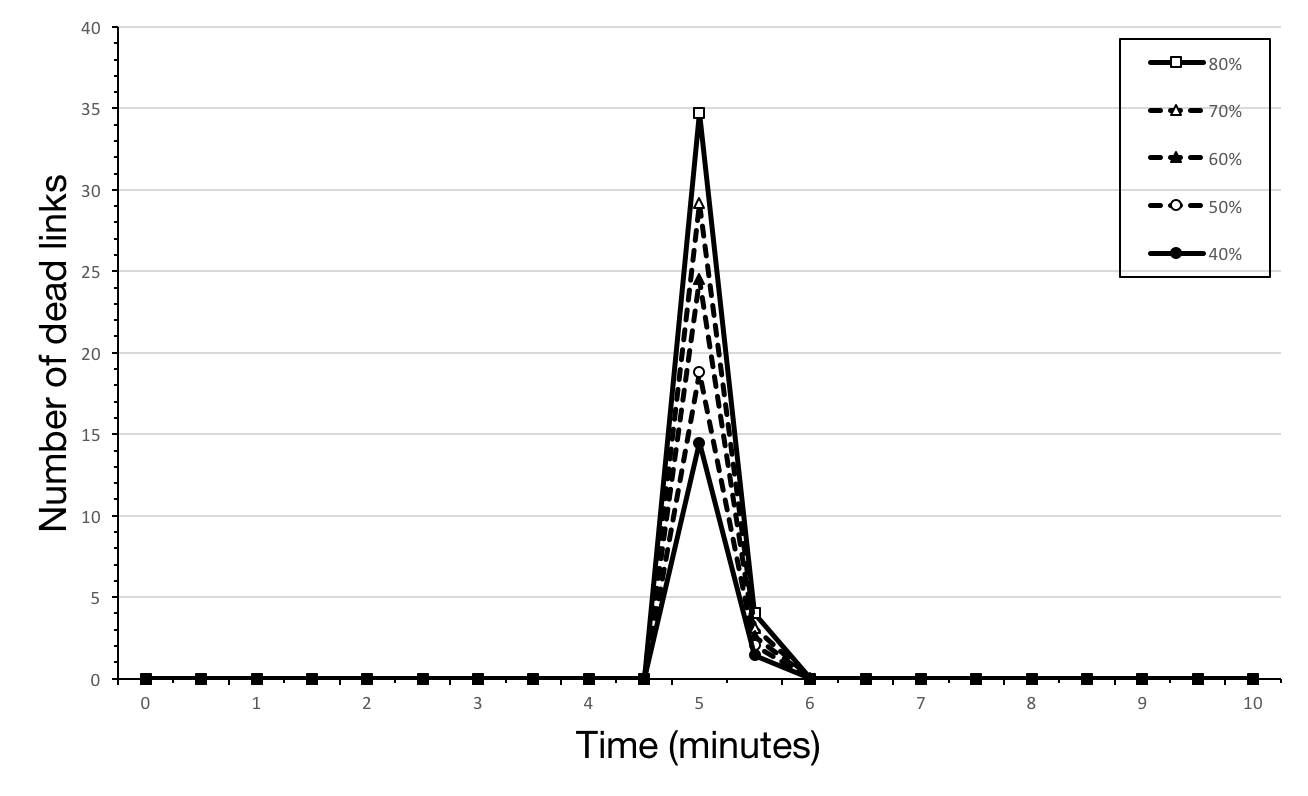
\includegraphics[keepaspectratio=true, width=1\linewidth]{images/average_dead_links}
  \caption{}
  \label{fig:average_dead_links}
\end{subfigure}%
\begin{subfigure}{.5\textwidth}
  \centering
  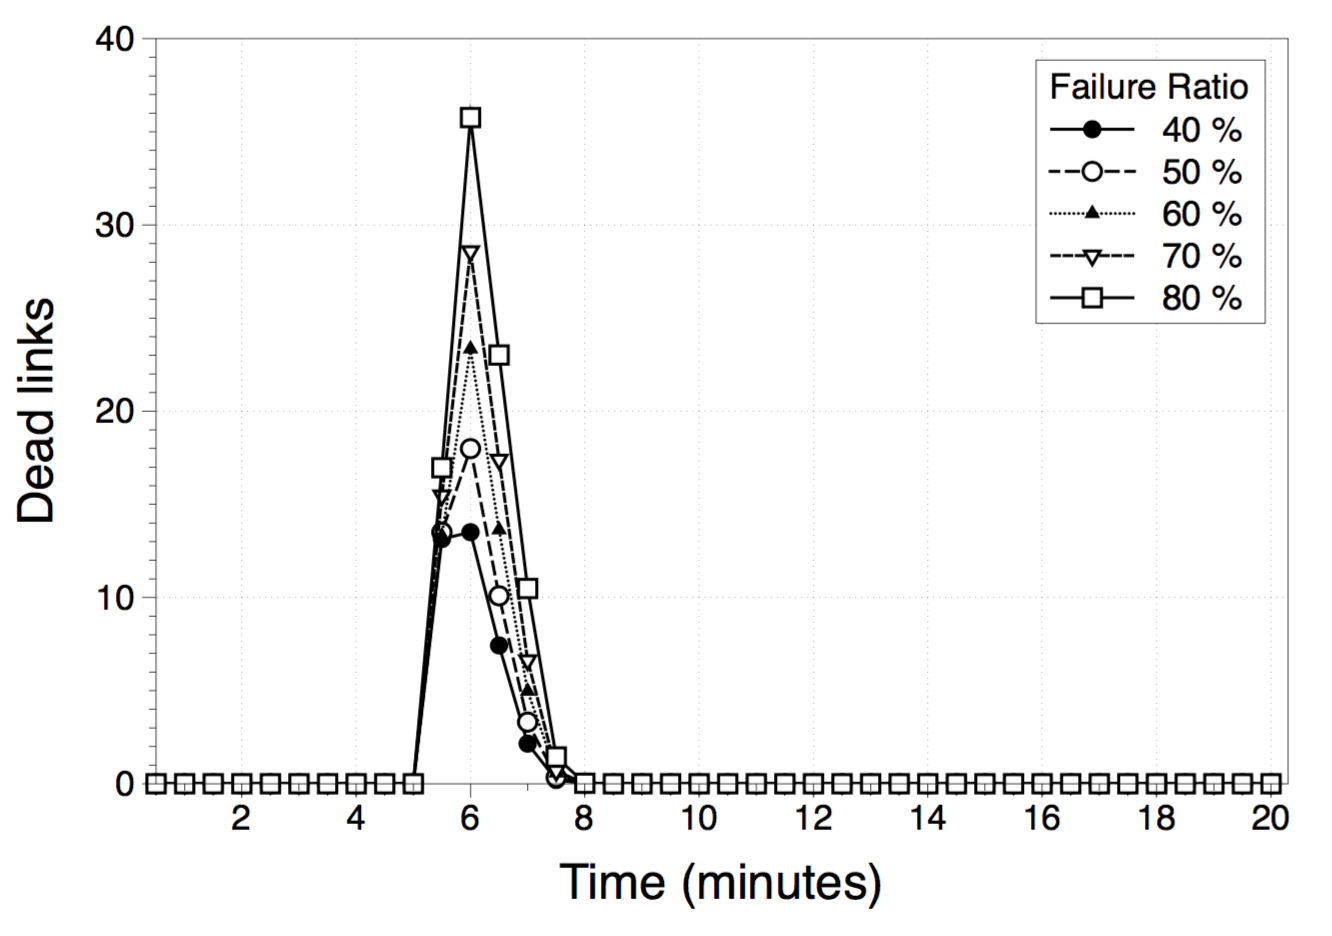
\includegraphics[keepaspectratio=true, width=1\linewidth]{images/paper_average_dead_links}
  \caption{}
  \label{fig:paper_average_dead_links}
\end{subfigure}
\caption{Average number of dead links in a flash crowd scenario.~\ref{fig:average_dead_links} represents our result,~\ref{fig:paper_average_dead_links} is the test reported in the paper.}
\label{fig:robustness_dead_links_failures}
\end{figure}

\newpage
In the last test shown in Figure~\ref{fig:robustness_hop_count_churn} we want to measure the robustness under different levels of churn, as they did in the original paper. We maintain the same timeout of 10 seconds and the same percentage of nodes that continuously join and leave. In Figure~\ref{fig:average_hop_count_churn_1impl} we notice that our implementation is robust to all the various levels of churn, even in a better way than the original. This is due to WebRTC: in fact we do not have a failure detector that captures the failure of a node (with the relative problematics), but is all handled inside the EasyRTC Framework. This give us the possibility to immediately capture the ``failure'' event and replace the broken link with a new one, without undermining the average hop count. In Figure~\ref{fig:average_hop_count_churn_2impl} we have the second implementation, and as we can notice the average is higher than the first implementation, although it is lower than the original represented in Figure~\ref{fig:paper_average_hop_count_churn}.

\begin{figure}
\centering
\begin{subfigure}{.5\textwidth}
  \centering
  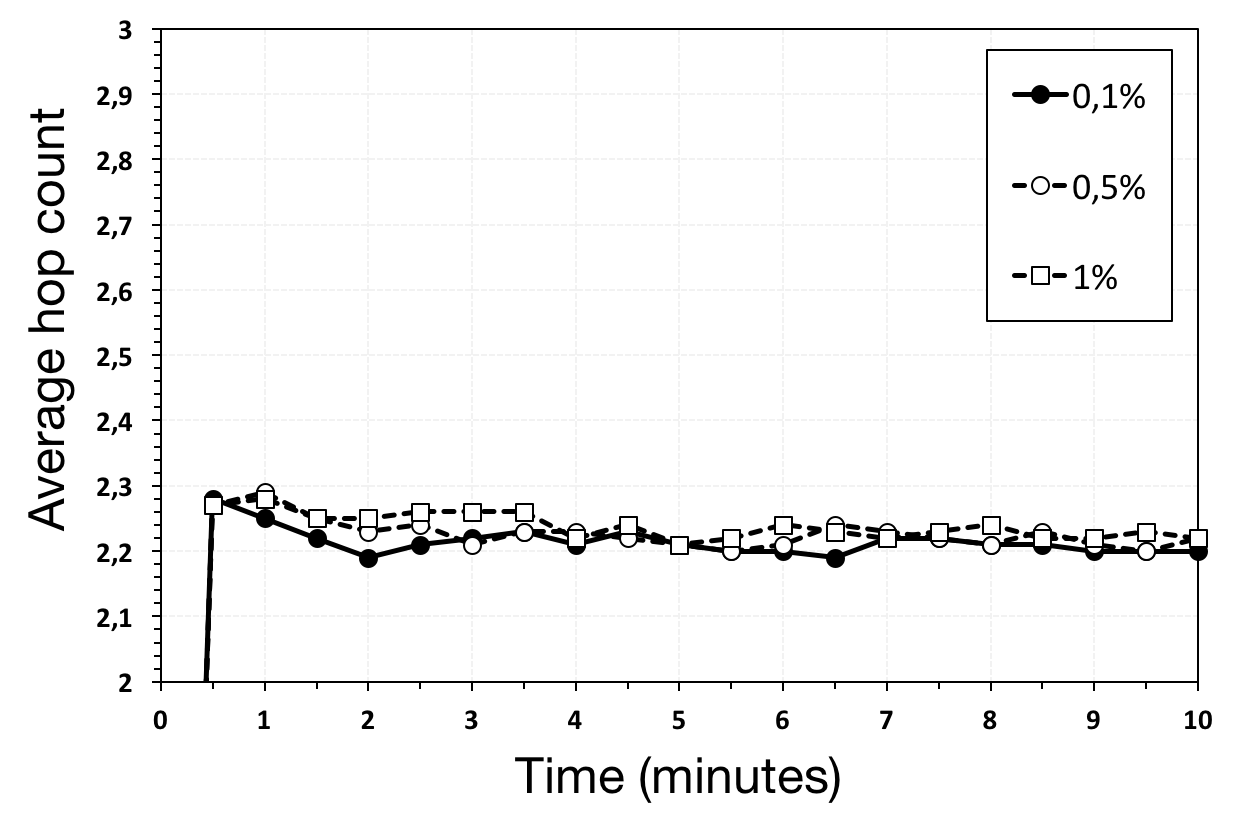
\includegraphics[keepaspectratio=true, width=1\linewidth]{images/average_hop_count_churn_1impl}
  \caption{}
  \label{fig:average_hop_count_churn_1impl}
\end{subfigure}%
\begin{subfigure}{.5\textwidth}
  \centering
  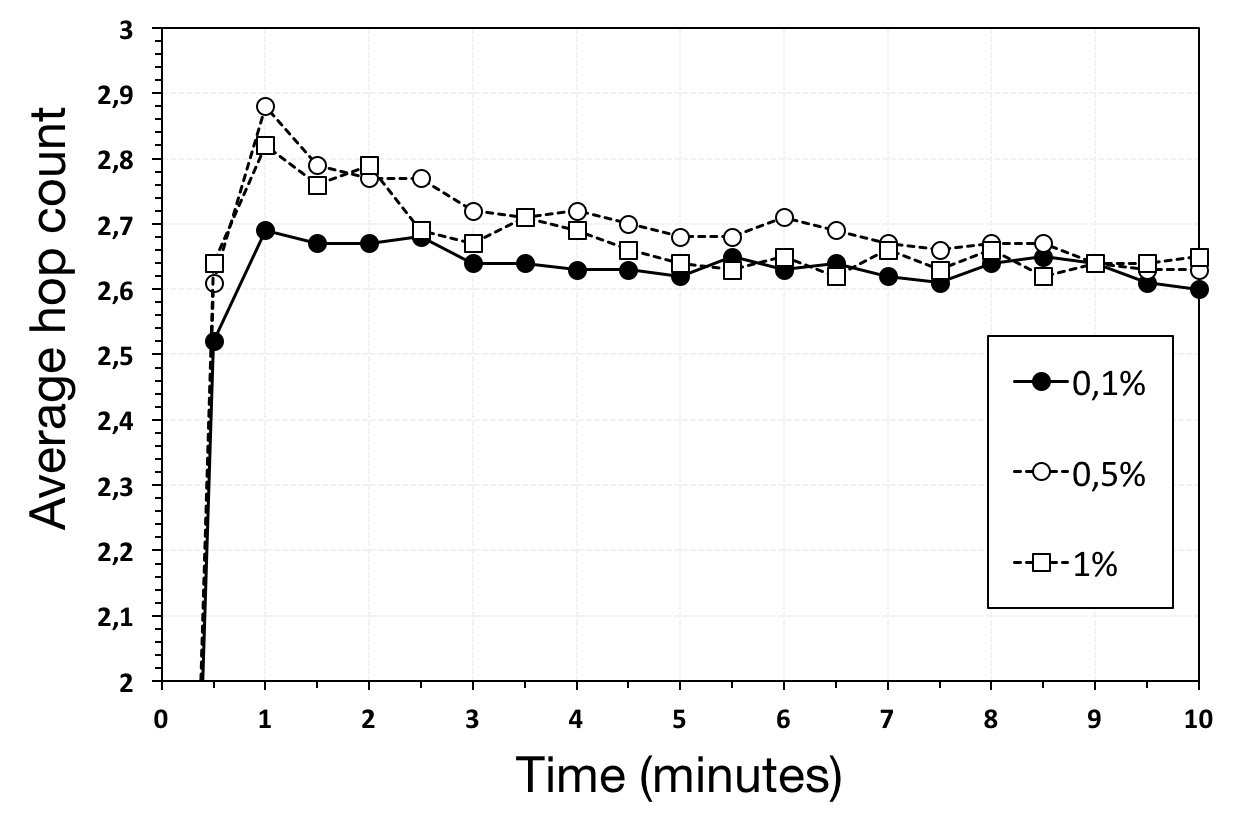
\includegraphics[keepaspectratio=true, width=1\linewidth]{images/average_hop_count_churn_2impl}
  \caption{}
  \label{fig:average_hop_count_churn_2impl}
\end{subfigure}
\begin{subfigure}{.5\textwidth}
  \centering
  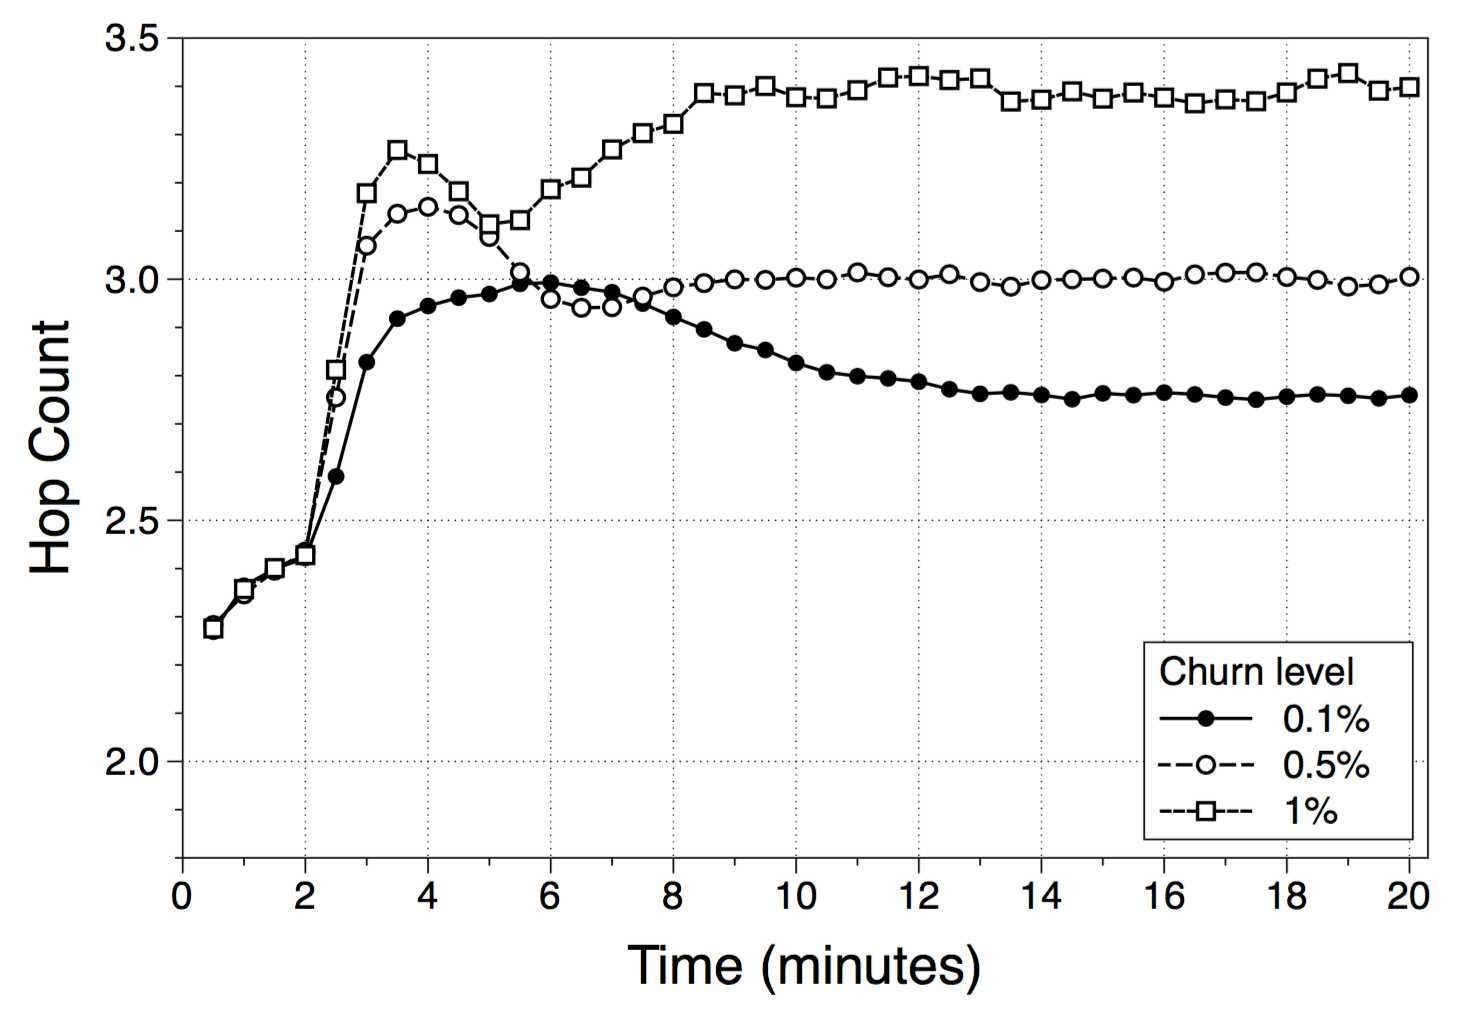
\includegraphics[keepaspectratio=true, width=1\linewidth]{images/paper_average_hop_count_churn}
  \caption{}
  \label{fig:paper_average_hop_count_churn}
\end{subfigure}
\caption{Average hop count under varying levels of churn. ~\ref{fig:average_hop_count_churn_1impl} represents our result in the first implementation (\getMetropolisHastingsNeighbour over all the connected peers),~\ref{fig:average_hop_count_churn_2impl} represent our result in the second implementation(\getMetropolisHastingsNeighbour over the base overlay) and~\ref{fig:paper_average_hop_count_churn} is the test reported in the paper.}
\label{fig:robustness_hop_count_churn}
\end{figure}

